\documentclass[fleqn,10pt]{wlscirep}
\usepackage[utf8]{inputenc}
\usepackage[T1]{fontenc}
\usepackage{caption}
\usepackage{subcaption}
\usepackage{setspace}
\usepackage{multirow}
\usepackage{epstopdf}
\usepackage{blindtext}
\usepackage{import}
\usepackage[percent]{overpic}
\usepackage{tabularx}
\usepackage{tikz}
\usepackage{hyperref}
\usepackage{float}
\usetikzlibrary{shapes.geometric, arrows}
\tikzstyle{startstop} = [rectangle, rounded corners, minimum width=3cm, minimum height=1cm,text centered, draw=black, fill=red!1]
\tikzstyle{textbox} = [rectangle, rounded corners, minimum width=3cm, minimum height=1cm,text centered, draw=white, fill=red!1]
\tikzstyle{io} = [trapezium, trapezium left angle=70, trapezium right angle=110, minimum width=3cm, minimum height=1cm, text centered,text width=2cm, draw=black, fill=blue!1]

\tikzstyle{process} = [rectangle, minimum width=3cm, minimum height=1cm, text centered, draw=black, fill=orange!1]

\tikzstyle{decision} = [diamond, minimum width=2.5cm, minimum height=1cm, text centered,text width=2cm, draw=black, fill=green!1]

\tikzstyle{arrow} = [thick,->,>=stealth]
%\tracinggroups=1
%\tracingnesting=2
%\showgroups






%\usepackage{fontspec}
%\setmainfont{Code2000}
\graphicspath{{./Plots/}}
\title{ Challenges in estimation of plot-scale emissivity and surface temperature using flux tower measurements} 

%\addbibresource{My_ref.bib}

\author[1,*]{Gitanjali Thakur}
\author[1]{ Stanislaus J. Schymanski}
\author[1]{Kaniska Mallick }
\author[1]{Ivonne Trebs}
\author[1]{Mauro Sulis}
\affil[1]{Luxembourg Institute of Science and Technology, ERIN, Belvaux, L-4422, Luxembourg}

\affil[*]{gitanjali.thakur@list.lu}
%SJS: If you want to use your own email-address, it might be wise to use one that will not expire when you finish your PhD. Otherwise, you could make me the corresponding author and I would then forward any emails to wherever you will be in a couple of years.
%GT: It is my first paper so, it is good if you are corresponding author as i will learn how to communicate with the journal editor.
%Instruction for writing the paper

%Scientific reports instruction for manuscripts:
%Your manuscript text file should start with a title page that shows author affiliations and contact information, identifying the corresponding author with an asterisk. We recommend that each section includes an introduction of referenced text that expands on the background of the work. Some overlap with the Abstract is acceptable.

%For the main body of the text, there are no specific requirements. You can organise it in a way that best suits your research. However, the following structure will be suitable in many cases:

    %Introduction
    %Results (with subheadings)
    %Discussion (without subheadings)
    %Methods

%You should then follow the main body of text with:

    %References (limited to 60 references, though not strictly enforced)
    %Acknowledgements (optional)
    %Author contributions (names must be given as initials)
    %Additional Information (including a Competing Interests Statement)
    %Figure legends (these are limited to 350 words per figure)
    %Tables (maximum size of one page)



%\keywords{Keyword1, Keyword2, Keyword3}

\begin{abstract}

Land surface temperature (LST) is a pre-eminent state variable that controls the energy and water exchange between the Earth’s surface and the atmosphere. At landscape scale, LST is derived from thermal infrared radiance measured using space-borne radiometers. At the plot-scale, flux tower recorded longwave radiation components is inverted  to retrieve LST. Since down-welling longwave component was not measured routinely for a long time a conventional practice is using stephan boltzmanfor the plot-scale LST retrieval (only up-welling longwave component) . This gives rise to the question if ignoring down-welling longwave radiation is adequate for plot-scale LST estimations. Another associated question is how to obtain the correct surface emissivity using  flux tower measurement needed for plot-scale LST retrievals . The current work addresses these two important questions using observations at ten eddy covariance towers having different land cover types. We found that the LST values obtained using up-welling and down-welling longwave component (long equation) are 0.5 to 1.5K lower than if only up-welling longwave components  were used (short equation). Plot-scale emissivity was estimated using observed sensible heat flux and estimated surface to air temperature difference. Plot-scale emissivity obtained using the complete equation was generally lower than if the simplified equation was used, for all land cover types. We also quantified the uncertainty in plot-scale LST and emissivity due to error in measured fluxes. We found that despite additional input data for the long equation, the uncertainty in plot-scale LST was not greater than if long equation was used. Landscape-scale day-time LST obtained from satellite data (MODIS TERRA) were strongly correlated with our plot-scale estimates, but on average higher by several degrees, regardless of the method of estimation. For most sites, the correspondence between MODIS LST and plot-scale LST estimates increased significantly if plot-scale emissivity was used instead of the landscape-scale emissivity obtained from satellite measurements. The implication of this work at ecosystem-scale (eddy covariance sites) can give an idea about the suitability of using aerodynamic and radiometric measurement in a common context (plot-scale emissivity estimation). 
%SJS: I re-wrote a bit for (hopefully) improved clarity and focus. Please check.



\end{abstract}
\begin{document}

\flushbottom
\maketitle
% * <john.hammersley@gmail.com> 2015-02-09T12:07:31.197Z:
%
%  Click the title above to edit the author information and abstract
%
\thispagestyle{empty}


\section*{Introduction}
%\subsubsection*{LST and net radiation (General statements about the field of research to provide the readers with a setting for the problem to be reported)}
%SJS: While reading, I realised that each of the SEB components can be negative or positive, so I re-wrote to be more general.
The surface energy balance (SEB) can be sub-divided into radiative components (often lumped in net radiation, $R_{net}$) and thermodynamic components, including sensible, latent heat flux ($H$, $LE$ respectively) and ground heat flux ($G$):
\begin{equation}\label{eq_seb}
R_{net} = H + LE + G 
\end{equation}
In this text, all energy balance components are expressed as power per horizontal surface area, in ($W m^{-2}$). %LST importance
As the surface to air temperature difference drives the exchange of sensible heat between surface and atmosphere, all components of Eq. (1) depend on the land surface temperature (LST). It directly affects the amount of emitted longwave radiation and it influences the saturation vapor pressure at the surface that drives latent heat flux. Thus, the ecohydrological functioning and carbon-water coupling are largely controlled by the surface temperature of the soil-vegetation system \cite{still2021imaging}. As it contains imprints of surface moisture variations and micro-climatic conditions within and above plant canopies, thereby controlling the magnitude and partitioning of the water and energy fluxes\cite{mallick2015reintroducing}. This makes LST of great importance to the modelling community. It is used to constrain climate models and weather prediction models \cite{zheng2012improvement,koch2016spatial}, as a prognostic variable in land surface models (LSM) and as diagnostic variable in surface energy balance models \cite{koch2016spatial,mallick2015reintroducing}. Therefore, it is crucial to have access to reliable estimates of LST over large spatial and temporal scales. 
%At the same time, the involvement of LST in the radiative energy balance components offers an opportunity for remote-sensing based monitoring of its spatial and temporal variation.

Net radiation ($R_{net}$) can be sub-divided into down-welling and up-welling components. Only a fraction of solar top-of-the-atmosphere radiation reaches the Earth's surface, as some is reflected back to space by clouds, some is absorbed by the atmosphere and emitted later as longwave radiation. Part of the longwave radiation emitted by the atmosphere reaches the surface as down-welling longwave radiation ($R_{ldown}$), along with the remaining down-welling shortwave radiation ($R_{sdown}$). At the surface, parts of down-welling shortwave and longwave radiation are reflected back to the atmosphere ($R_{sref}$ and $R_{lref}$, respectively), and the rest is absorbed. In addition to reflecting radiation, the surface is also emitting longwave radiation as a function of surface temperature ($T_s$, K) and surface emissivity ($\epsilon$) following the Stefan-Boltzmann (SB) equation:
\begin{equation}\label{eq_Rlem}
R_{lem}= \epsilon \sigma T_{s}^{4}
\end{equation}
where $\sigma$ ($Wm^{-2}K^{-4}$) is the SB constant. 
Putting the radiative components together, we can sub-divide $R_{net}$ into:
\begin{equation}\label{eq_Rn1}
R_{net} = R_{sdwn} + R_{ldwn} - R_{sref} - R_{lref} - R_{lem}
\end{equation}
Reflected shortwave in Eq. ({\ref{eq_Rn1}}) is can be expressed as $R_{sref} = \alpha R_{sdown}$, where $\alpha$ is the surface albedo. Similarly, reflected longwave is a function of down-welling longwave and surface emissivity ($\epsilon$) and expressed as:
\begin{equation}\label{eq_Rlref}
R_{lref} = (1 - \epsilon) R_{ldwn} 
\end{equation}
LST or radiometric temperature can be estimated from the infrared radiance emanating from a given surface\cite{kustas2007utility}. The emitted and down-welling longwave radiance are measured by an infrared radiometer at given angle within its instantaneous field of view (fov). The radiation received by a pyrgeometer or infrared sensor is a combination of the radiation emitted and reflected by the surfaces in the field of view. Thus, LST estimated from an infrared measurement is the “ensemble directional radiometric surface temperature”, representing the ensemble of various surface elements present within the sensor's instantaneous fov \cite{norman1995terminology}. A downward facing sensor relatively close to the surface (a few meters for an eddy covariance tower) essentially measures up-welling longwave radiation ($R_{lup}$) from the surface, which is the sum of emitted and reflected longwave radiation:
%This radiant energy can be attenuated, absorbed, and re-emitted by the atmosphere between the surface and the sensor before reaching the sensor \cite{krishnan2020intercomparison}
\begin{equation}\label{eq_Rlup}
R_{lup} = R_{lem} + R_{lref}
\end{equation}
Substitution of Eqs. \ref{eq_Rlref} and \ref{eq_Rlem} into Eq. \ref{eq_Rlup} yields $R_{lup}$ as a function of emissivity, surface temperature and down-welling longwave radiation:
\begin{equation}\label{eq_leq}
R_{lup}= \epsilon \sigma T_{s}^{4} + (1- \epsilon)R_{ldwn}
\end{equation}
The above equation can be solved for surface temperature as a function of measured longwave and known surface emissivity:
\begin{equation}\label{eq_Tleq}
T_{s} = \sqrt[4]{\frac{R_{ldwn}}{\sigma} - \frac{R_{ldwn}}{\epsilon \sigma} + \frac{R_{lup}}{\epsilon \sigma}}
\end{equation}
where, $\epsilon$ is the surface emissivity ranging between 0 and 1, $\sigma$ ($Wm^{-2}K^{-4}$) is the Stefan-Boltzman constant and $T_{s}$ ($K$) is the LST. %SJS: What do you mean by ensemble? Is this different to the previous definition of the same parameters? If the same, I would remove the above lines.%GT: yes, I wrote this to remind the reader:it is effective emissivity means representative of the combination of surfaces radiaometers field of view 
Emissivity is defined as efficiency of a surface to emit thermal energy relative to a perfect black body. It  depends on surface morphology, soil moisture, soil chemistry, roughness, spectral wavelength, temperature and view angle\cite{norman1995terminology}. %SJS: really temperature? But then we would have temperature on both sidds of eq_Tleq.%GT:yes, following plancks law, total energy radiated increases with temperature while the peak of the emission spectrum shifts to shorter wavelengths. 
The radiative energy  emitted at a specific wavelength is related to its temperature using Planck's function\cite{wang_estimation_2005-1}. The emissivity of a land surface (composed of various grey body) is retrieved  using radiative transfer models\cite{hulley_quantifying_2012-1,jin2006improved,wang_evaluation_2009}. Thermal remote sensing (MODIS) is used to measure spectral emissivity through four channels (28, 29, 30, 31) at wavelengths ranging between 8-12 $\mu$m \cite{jin_improved_2006-1} and the system of equations iteratively solved for a given range of wavelengths (9 - 12$\mu$m) to obtain $\epsilon$ and LST.


In last two decades, plot-scale radiometric data collected at eddy covariance sites (ECS) have gained popularity for in-situ LST retrieval due to its high spatial and temporal resolution. In addition to this the land cover specificity is also an important factor as the LST estimates are of relatively homogeneous footprint in comparison to MODIS pixels. These measurements are primarily use to assess the impacts and feedbacks of climate change on key ecosystem fluxes\cite{baldocchi2001fluxnet}. In order to invert LST as shown in Eq. \eqref{eq_Tleq}, $\epsilon$ values are required. However, the surface emissivity of the tower footprint cannot be estimated using radiative transfer models as radiometers do not measure spectral bands separately to deduce emissivity directly. 
%which can be obtained from MODIS,classification table \cite{humes1994variability} or can be calculated for at plot-scale using flux tower measurement \cite{maes2019potential, holmes_cloud_2016, holmes_land_2009}.%SJS: What do you mean by ensemble? Average?
%GT: equivalent or effective emissivity of various surfaces%\subsubsection*

By definition, LST is a thermodynamic temperature that can be felt or measured by an accurate thermometer at the land surface-atmosphere point-of-contact and is independent of wavelength \cite{guillevic2017land}. The instantaneous value of LST is the result of interplay between the net radiation at the surface, ground heat flux and turbulent fluxes of heat ($H$) and moisture ($LE$) \cite{wang_global_2013-2}. Thus, LST can also be used for the estimation of the sensible heat flux \cite{sun1995relationship} and latent heat flux \cite{jacob2001comprehensive} between the surface and the atmosphere. For plot-scale emissivity retreival we focus on $H$, which is defined as heat transfer driven by a surface to air temperature difference. It can be expressed mathematically in analogy to Ohm's law as:
\begin{equation}\label{eq_H1}
H= \rho C_{p}(T_{s} - T_{a})/r_{a}
\end{equation}
\begin{equation}\label{eq_H}
H= m(T_{s} - T_{a})
\end{equation}
where $T_{a}$ (K) is the temperature of the air measured at some height above the surface, $C_{p} (J kg^-1 K^-1)$ is the specific heat capacity of air, $\rho (kg (m)^-3)$ is the air-density, $r_{a}(S m-1)$ is the total resistance to heat transport from surface to the atmosphere. $m (m/s)$ is a proportionality constant obtained by lumping $(\rho C_{p}/r_{a})$ and can be broadly referred as heat transfer coefficient. $m$ depends on surface characteristics and micro meteorology \cite{lhomme_radiative_1988}. It is evident from Eq. (\ref{eq_H}), that for $T_{s} - T_{a} = 0 $ ($\Delta$T=0), $H$ will be zero. This boundary condition and the linearity of $H$ and $\Delta T $ relationship is used to estimate $\epsilon$ at the plot scale from observed of $H,T_a$ and estimated $T_{s}$ using measured longwave \cite{holmes_land_2009,holmes_cloud_2016-1,maes2019potential}. %heterogenous nature of vegetated land surface 
%SJS: You should explain a bit more how H, T_a and longwave are used to get an estimate of epsilon. Just in general here, and in more detail in the Methods, where it is not explained at all.
%GT: I have explained %\subsection*{explaining H= K(T_{s} - T_{a})+c}

However, due to surface heterogenity sparse canopy is prone to footprint mismatch between the aerodynamic (flux tower) footprint and radiometric (hemispherical) footprint \cite{chu2021representativeness,marcolla2018geometry,morillas2013using} which can result into a different boundary condition i.e at $\Delta T =0, H \not= 0$. Aerodynamic footprint represents the area contributing to measured sensible heat, air temperature and the hemispherical footprint is the area within radiometric FOV contributing to the measured longwave (used for $T_{s}$ estimation). For instance if the radiometer fov has more tree crowns and less soil in comparison to the flux tower footprint the observed longwave will have a bias. In this kind of scenario we would expect a non zero H for 0 $\Delta T$. In order to capture such a bias in plot-scale $\epsilon$ estimation we allowed $H(\Delta T)$ linear regression to have an intercept (c) as shown in Eq. \ref{eq_H2}.
\begin{equation}\label{eq_H2}
H= m(T_{s} - T_{a}) \pm  c(H)
\end{equation}
H is representative of the sensible heat flux from eddy covariance tower footprint,$T_{s}$ is representative of all the radiating surfaces in the sensor’s view. C is interpreted as the $H$ from aerodynamic footprint which is not seen by the radiometer. For example if the mismatch in footprint is a hotter area relative to the shared foot print of the measuring devices  i.e. dry soil patch then $H(\Delta T)$ relationship can be represented by adding a negative intercept to the $H (\Delta T)$ relationship. Similarly if the footprint mismatch is a relatively colder area i.e leaves in shade the regression can have a positive intercept.

%Water-limited ecosystems are more prone to mismatch of tower flux footprint and hemispherical radiometric footprint due to their heterogeneous vegetation composition as compared to the mesic ecosystems (Marcolla and Cescatti, 2018; Morillas et al., 2013)

%\subsection*{Lst estimation using remote sensing}
%Since the 1990s, improvements in infrared thermometrics have resulted in various advancements for the estimation of LST and emissivity using remote sensing \cite{wang_estimation_2005-1}. Remotely sensed thermal data is capable of fully characterizing the daily cycle of LST at the regional scale. The thermal radiance from the land surface is obtained using space-borne instruments consisting of radiometers. The radiative energy  emitted at a specific wavelength is related to its temperature using Planck's function \cite{wang_estimation_2005-1}. Since LST and emissivity are closely coupled\cite{hulley_quantifying_2012-1,jin2006improved,wang_evaluation_2009} the use of Planck's function for natural surfaces (grey bodies) makes the system under-determined as emissivity is unknown. Thus, radiative transfer models are used to solve the under-determined system of equations iteratively to obtain emissivity and LST for a given range of wavelengths (9 - 12$\mu$m). MODIS measures spectral emissivity through four channels (28, 29, 30, 31) at wavelengths ranging between 8-12 $\mu$m \cite{jin_improved_2006-1}. The final LST is obtained by the cumulative sum of radiative energy obtained at different wavelengths using Eq. (\ref{eq_leq}) with derived emissivity for crossponding wavelength\cite{jimenez2006emissitivity}.
%SJS: I find the above difficult to understand. We should get help from Ivonne and Kanishka to describe this better, or even remove the whole paragraph as it is not too relevant for your study, which deals with plot-scale estimates.
%GT: it deals with plot scale but I m comparing plot-scale LST with remotely sensed data as a refrence so it is better i give reader a background of how lst and emissivity is estimated in remote sensing

%\subsection*{Lst estimation using flux tower}
%In last two decades, plot-scale radiometric data collected at eddy covariance sites (ECS) have gained popularity for in-situ LST retrieval due to its high spatial and temporal resolution. In addition to this the land cover specificity is also an important factor as the LST estimates are of relatively homogeneous footprint in comparison to MODIS pixels. These measurements are primarily use to assess the impacts and feedbacks of climate change on key ecosystem fluxes\cite{baldocchi2001fluxnet}.
%The measurements are publicly available through different networks, e.g., SURFRAD (https://esrl.noaa.gov/gmd/grad/surfrad/), FLUXNET (https://fluxnet.org/) or TERN (http://www.ozflux.org.au/monitoringsites/). Most ECS record high quality surface longwave radiation data using tower-mounted radiometers, infrared thermometers or pyrgeometers. The range of measurement wavelengths for infrared thermometers ranges between $6.5 and 14 µm$
%SJS: Below, I try to motivate the use of $H$ for plot-scale LST retrieval, to improve the flow.
%The disadvantage is that the surface emissivity of the tower footprint cannot be estimated using radiative transfer models as radiometers do not measure spectral bands separately to deduce emissivity directly.
Plot-scale $\epsilon$ estimation using observed $H, T_{a}, R_{lup}, R_{ldw}$ as described above, may be fraught with substantial uncertainty. As it is unclear how error in observed fluxes propagates into the uncertainty of  estimated LST and $\epsilon$. The turbulent fluxes of $H$ measured at the ECS are averaged over smaller time (30 or 60 minutes) and the averaging over this time interval is typically dominated by random errors \cite{rannik2016random, mauder2020surface}. The other source of error is the radiation measurement which can vary between sites, due to the difference in accuracy and precision of the in-situ radiometers or pyrgeometer, differences in field of view (FOV), wavelength bands, and spectral response functions of the sensors. For reference, the accuracy of dedicated infrared temperature (IRT) sensors is given by their manufacturers as $0.5$K, but it is not clear what sources of uncertainty are considered in this estimation \cite{vickers2010uncertainty}.
%The uncertainty in Eddy-covariance (EC) measurements can be attributed to random errors from turbulence and systematic errors from signal noise \cite{mauder2013strategy}. Unclosed energy balance and limited footprint essentially leads to systematic errors
 %because of the stochastic nature of turbulence and also due to the noise present in the measured signals
%easily be obtained from satellite-based measurements due to the footprint mismatc 
%The longwave flux is a direct function of the physical temperature of the land surface,.
 %SJS: Did I get this right?
 %GT:yes, Thank you
%\subsection*{Uncertainities in flux tower measurement}
%also instrument calibration, unmet methological challenges, and data processing can result into systematic error \cite{mauder2013strategy}. Therefore, it is important to quantify the uncertainity introduced in emissivity estimation considering the error bounds (systematic error or bias) in $R_{lup}$, $R_{ldwn}$, $H$ and $T_{a}$ 
%is shown in Fig. (\ref{fig:eps_unc1}a). 
%SJS: The above is the motivation for the analysis and should be in the Intro, not in the Results. 
% GT: It was Stan's suggestion that I should work on the  text of uncertainty analysis using  table 4.8 of Thomas fokens book which suggests about the maximum  limit of the error in measured fluxes, which is about 35 watt/m2. 
 %SJS: Are you sure that signal noise leads to non-random, systematic errors? Or do you mean instrument drift?
 %GT:All eddy-covariance flux measurements are asso-ciated with random uncertainties which are a combination of sampling error due to natural variability in turbulence and sensor noise. 
%GT Vickers et.al. (2010)
 %Systematic errors can be minimised by properly calibrating and maintaining the instruments \cite{munger2012measurement} and by applying all required corrections and conversions for EC to one comprehensive post-processing strategy \cite{leuning2012reflections}. However, the systematic error estimation is not included in the automatic processing. As a result of which in-situ $\epsilon$ estimated using EC measurements are prone to a certain level of uncertainty. Therefore, quantification of uncertainity is important for reliable estimate of $\epsilon$. 
 %SJS: I commented out the above, as I don't think the exact processing steps in the EC data are relevant here. Could you just give a rough quantification of the error in H?
 %SJS: Can you provide a reference? 
  %Some of the issues related to quality control and flux sampling problems are addressed by using extensive suite of algorithms (Vickers and Mahrt (1997, hereafter VM97), Papale et al. (2006)).. 
%\subsubsection*{The importance of reflected longwave}
By design, IRT sensors only measure upwelling infrared radiance and therefore cannot explicitly account for the amount of reflected down-welling infrared radiation in the signal. For a long time, down-welling longwave $R_{ldw}$ was not routinely observed at ECS \cite{wang_evaluation_2009-1} and was also considered to be the most poorly quantified component of the radiation budget \cite{trenberth2012tracking}. Therefore, the second term in Eq. (\ref{eq_leq}) is commonly omitted, arguing that $\epsilon\approx 1$, and therefore Eq. (\ref{eq_leq}) is simplified to \cite{crago_use_2014-3}:
\begin{equation}\label{eq_seq}
R_{lup} \approx \epsilon \sigma T_{s}^{4}
\end{equation} 
Eq. \ref{eq_seq} can be solved for $T_s$ to yield what we will term the "short equation" (SEQ) for $T_s$:
\begin{equation}\label{eq_Tseq}
T_{s} \approx \sqrt[4]{\frac{R_{lup}}{\epsilon \sigma}}
\end{equation} 
Note that the above derivation is actually flawed, as the second term of Eq. (\ref{eq_leq}) was omitted arguing that $\epsilon\approx 1$, and yet $\epsilon$ was retained in the first part of the equation. Nevertheless, even with the availability of down-welling longwave measurements \cite{stephens1995review}, the use of Eq. (\ref{eq_seq}) is still a common practice\cite{crago_use_2014-2}. This gives rise to the question if the short equation (Eq. \ref{eq_Tseq}) is adequate to estimate LST from ground-based measurements. In the remainder of this paper, we will refer to LST obtained using the complete or "long equation" (Eq. \ref{eq_Tleq}) as $T_{leq}$ and to LST obtained using the simplified or short equation (Eq. \ref{eq_Tseq}) as $T_{seq}$.

%\subsection*{Purpose and objectives of this study}
%SJS: Does SciRep allow sub-sections in the intro? If so, I would introduce a few above, and definitely uncomment this subsection heading.
%GT:no in sci repo no subsection for introduction is allowed

In the present study, we evaluate and analyse the differences in plot-scale LST and emissivity estimated using the complete (Eq. \ref{eq_Tleq}) and short (Eq. \ref{eq_Tseq}) equations. 
The following research questions are addressed:
\begin{enumerate}
	\item Is the short equation (Eq. \ref{eq_Tseq}), neglecting the reflected down-welling longwave radiation, adequate to estimate LST from ground-based measurements?
	\item Does the estimation of plot-scale $\epsilon$ based on observed sensible heat flux $H$ has an advantage over satellite derived $\epsilon$ for LST estimation?
    %\item Does accepting an intercept in $H (\Delta$ T) lead to realistic estimate of plot-scale $\epsilon$?
    \item How much uncertainity is introduced in plot-scale LST and $\epsilon$ due to errors in measured fluxes?
    
\end{enumerate}    
To answer these questions, we analysed data for 10 eddy covariance sites in different biomes and climates (see Table \ref{table:studysites}).
Plot-scale broadband monthly emissivity was derived using observed $H$ and estimated $\Delta T$ as proposed by Holmes et al. \cite{holmes_land_2009}.  Plot-scale LST was estimated using plot-scale or landscape-scale emissivity with (Eq. \ref{eq_Tleq}) and (Eq. \ref{eq_Tseq}). Plot-scale LST were compared with MODIS LST ( TERRA satellite-sensed) for the times of satellite over-pass. Uncertainty in emissivity and LST due to error in observed fluxes was calculated using SOBOL based uncertainty analysis (SAlib) \cite{rosolem2012fully}. %SJS: Need to provide references for SOBOL and SAlib.%GT added ref.
 %SJS: Please complete this sentence, and
See the Methods section for more details.

\section{Results}
%SJS: In the main text of the results section, you should describe the important features of the results, i.e. the take-away messages that you will come back to during the discussion.

%Details needed to understand each figure should be provided in the respective figure caption. I will try to re-write the below to give an example.
%SJS: I re-ordered the results, as I think it flows better to start with the comparison with Holmes and then present the other sites and comparison with MODIS LST.
\subsection{Plot-scale $\epsilon$ using complete and simplified equation}

Following the method proposed by Holmes et al. \cite{holmes_land_2009, holmes_cloud_2016}, plot-scale monthly emissivity ($\epsilon$) was estimated at the study site by fitting $\epsilon$ to minimise the root mean square error (RMSE) of the regression between $H$ and $\Delta T = T_s - T_a$ for every month using filtered measurements (based on net radiation  and wind speed). In Fig. \ref{fig:HDT}a, c, and d, we reproduced the original data of Figs. 2a, 3C, and 3Q in Holmes et al. (2009) \cite{holmes_land_2009} to validate our interpretation of their approach using the simplified equation (Eq. \ref{eq_Tseq}). We noted only marginal differences between the two results based on the short equation which are likely due to data filtering and fitting algorithms. The replication of the $H (\Delta T)$ plot using the complete equation (Eq. \ref{eq_Tleq}) in their analysis is given in Fig. \ref{fig:HDT}b. The use of complete equation (Eq. \ref{eq_Tleq}) resulted in substantially lower values of $\epsilon$ (10\%) as compared the values estimated by Holmes et al\cite{holmes_land_2009} for the common study sites (Brookings, Yatir Forest) (Fig. \ref{fig:HDT}c and d). Note that the complete equation also yielded $H(\Delta T)$ relationship for many more months at Yatir Forest than the short equation (Fig. \ref{fig:HDT}d), as it resulted in achieving a strong correlation between $H$ and $\Delta T$, which is one of the filtering criteria for the approach. The retrieved LST values were slightly higher (compare Panels a and b in Fig. \ref{fig:HDT}). The pattern of low $\epsilon$ and high LST using the complete equation compared to the simplified equation was confirmed for all 10 sites used in the present study (Table \textbf{SI 2}).
\begin{figure}[h!]
	\centering
	\begin{overpic}[width=0.45\textwidth]{Brookings_se_2005-08} 
		\put (19,61){\textbf{a}}
	\end{overpic}
	\begin{overpic}[width=0.45\textwidth]{Brookings_le_2005-08} % ,grid,tics=10
		\put (19,61){\textbf{b}}
	\end{overpic}
	\begin{overpic}[width=0.45\textwidth]{Brookings_emmi_twoequ} % 
		\put (19,59){\textbf{c}}
	\end{overpic}
	\begin{overpic}[width=0.45\textwidth]{Yatir_emmi_twoequ} % 
		\put (19,59){\textbf{d}}
	\end{overpic}
	\setlength{\belowcaptionskip}{-3ex}
	\caption{Reproduction of analysis presented in Figs. 2 (a) and 3 C and Q in Holmes et al. (2009) \cite{holmes_land_2009}. \textbf{(a)} Sensible heat ($H$) vs. $\Delta T = T_{seq} - T_{a}$ based on the short equation ($T_{seq}$, Eq. \ref{eq_Tseq}); (b) $H$ vs. $\Delta T$ based on the complete equation ($T_{leq}$, Eq. \ref{eq_Tleq}). Both show data for August 2005 at Brookings. Blue crosses mark data points satisfying the filtering criteria while black dots mark points not considered in the analysis. N is the number of blue crosses used for regression (red line), m is the slope of regression, RMSE is the root mean square error and $R^{2}$ is the coefficient of determination. The fitted $\epsilon$ value is reported in the title. \textbf{(c)} Optimised $\epsilon$values at Brookings obtained for the months where  $R^{2} > 0.5$ using the short equation (Eq. \ref{eq_seq}, black dots) and complete equation (Eq. \ref{eq_leq}, blue stars).  \textbf{(d)} Same as (c), but for Yatir Forest. See Table \ref{table:studysites} for site descriptions.}
	\label{fig:HDT}
\end{figure}
\subsection{Landscape scale vs plot-scale estimates of $\epsilon$ and LST}
At each site, LST was estimated using both the short equation ($T_{seq}$, Eq. \ref{eq_Tseq}) and the long equation ($T_{leq}$, Eq. \ref{eq_Tleq}). In the first step, tower-based longwave measurement  and landscape-scale  broadband $\epsilon$ from MODIS ($\epsilon_{MODIS}$, Eq. \ref{eq_emodis}) was used. The yearly daytime surface to air temperature difference for each study site is estimated is shown in Fig. \ref{fig:long_short_eq_epsilon_MODIS}. At all sites, Eq. \ref{eq_Tseq} resulted in higher day-time plot-scale $T_{s}$ estimates as compared to Eq. \ref{eq_Tleq}, when using $\epsilon_{MODIS}$, with the medians of surface-air temperature differences ($\Delta T$) differing by 0.8 to 1.5 K (Fig. \ref{fig:long_short_eq_epsilon_MODIS}). The difference in $\Delta T$ using two equation is highest at the water limited sites e.g AS, YA. Note that for two sites (LF and HS), the median values of daytime $\Delta T$ are negative.

\begin{figure}[h!]
	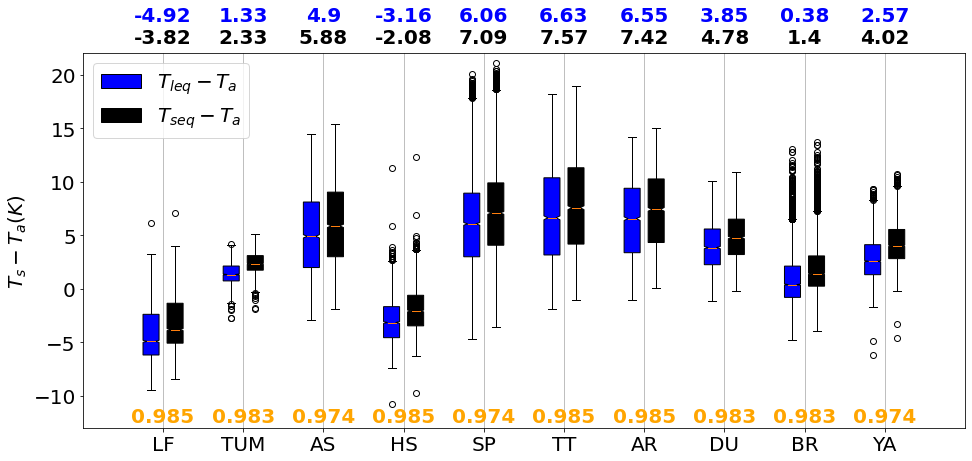
\includegraphics[scale=0.35]{Ts_Talocalleqseq.png}
	\centering
    \caption{
     Yearly distributions of half-hourly surface to air temperature differences ($\Delta T = T_s - T_a$) for a representative year at each site.  %SJS: what year? Daily, hourly, half-hourly? I just guessed here.
    %GT yes, it is half an hourly 
    LST are inverted using short and long equation (Eq. \ref{eq_Tseq}), Eq. \ref{eq_Tleq}) with landscape-scale emissivity ($\epsilon_{MODIS}$).
    The median values of $\Delta T$ are shown at top of the plot and the emissivities used for the $T_{s}$ retrieval are shown at the bottom in orange. See Table \ref{table:studysites} for site abbreviations.}
	\label{fig:long_short_eq_epsilon_MODIS}
\end{figure}
Comparison of estimated plot-scale LST using $\epsilon_{MODIS}$ at satellite overpass time with landscape-scale LST ($T_{MODIS}$) revealed strong correlations between plot-scale and landscape-scale LST estimates as shown in Fig. \ref{fig:LST local and MODIS}a, b. Use  of plot-scale $\epsilon_{plot}$ for plot-scale LST estimation ($T_{seq}$ and $T_{leq}$) resulted in substantial reduction of the bias as shown in Fig. \ref{fig:LST local and MODIS}c, d. This trend in bias reduction was similar to other sites (Table \textbf{SI2} for details). The  minimum bias is found  at the Tumbarumba a closed canopy (eucalyptus forest) and highest bias was obtained at Litchfield and Howards Springs an sparse canopy (woodland savanna). However, for some sites, weak correlation between satellite-derived and local LST estimates were also evident (at DU, $R^2$ was reduced from 0.8 to 0.4, see Table \textbf{SI2}). Also, using plot-scale $\epsilon$ for LST estimation resulted in positive $T_{s} - T_{a}$ at LF and HS as shown in \textbf{SI3}.  
\begin{figure}[h!]
	\begin{subfigure}{\textwidth}
		\begin{overpic}[width=0.45\textwidth]{As_epsmodis_seq_modis2017} % ,grid,tics=10
			\put (20,57){\textbf{a}}
		\end{overpic}
		\begin{overpic}[width=0.45\textwidth]{as_modiseps_leq_modis2017} % ,grid,tics=10
			\put (20,56){\textbf{b}}
		\end{overpic}
	\end{subfigure}


	\begin{subfigure}{\textwidth}
		\begin{overpic}[width=0.45\textwidth]{AS_optps_seq_modis2017} % ,grid,tics=10
			\put (20,55){\textbf{c}}
		\end{overpic}
		\begin{overpic}[width=0.45\textwidth]{AS_optps_leq_modis} % ,grid,tics=10
			\put (20,55){\textbf{d}}
		\end{overpic}
	\end{subfigure}
	\setlength{\belowcaptionskip}{-3ex}
	\caption{Landscape-scale LST ($T_{MODIS}$ derived from MOD11A1) vs. plot-scale LST at Alice Springs for 2016-2018. 
		\textbf{(a)} $T_{seq}$ based on short equation (Eq. \ref{eq_Tseq}) and satellite-derived (MODIS) landscape-scale broadband emissivity;
		\textbf{(b)} Same as (a), but $T_{leq}$ based on complete equation (Eq. \ref{eq_Tleq});
		\textbf {(c)} $T_{seq}$ based on short equation (Eq. \ref{eq_Tseq}) and monthly plot-scale emissivity;
		\textbf {(d)} Same as (c), but $T_{leq}$ based on complete equation (Eq. \ref{eq_Tleq}).
		Bias is mean $T_{seq} - T_{MODIS}$, N is the number of daily overpasses of MODIS between 2016 and 2018, c is the intercept, m the slope, RMSE is the root mean square error and $R^{2}$ is coefficient of determination. At each site, LST was estimated using both the short equation ($T_{seq}$, Eq. \ref{eq_Tseq}) and the long equation ($T_{leq}$, Eq. \ref{eq_Tleq}). In a first step, we used satellite-derived landscape-scale broadband emissivity from MODIS ($\epsilon_{MODIS}$, Eq. \ref{eq_emodis}) for estimating plot-scale LST from tower-based longwave measurements, and compared these with landscape-scale LST extracted from daily MODIS LST images ($T_{MODIS}$)
		%SJS: Could you clarify if R2 is not the coefficient of determination if whether bias is Mean(Ts) - Mean(T_MODIS) or Mean (Ts - TMODIS)?
		%bias is Mean (Ts - TMODIS) 
	}. 
	\label{fig:LST local and MODIS}
\end{figure}

\subsection{Plot-scale $\epsilon$ estimation considering footprint mismatching of measurement devices}
In order to account for the discrepancy in plot-scale $\epsilon$ estimation due to footprint mismatch of measuring devices $H$ vs. $\Delta T$ relationship was allowed to accept an intercept as shown in Fig. \ref{fig:2_mx_c}. The plot-scale $\epsilon$ using long equation with an intercept results into the conventional (realistic) range of emissivity in comparision to the one with no intercept at study sites as shown in Table (\ref{table:eps_comp}). The intercept value for Brookings, a grassland is 12\% of maximum sensible heat flux ($H_{max}$) and  for a mulga shrubs like AS is 20\% of $H_{max}$. The intercept value for HS is 70\% of $H_{max}$  and for Tum is 7\% of $H_{max}$. The intercept value is lowest for a  forest site (closed canopy) and highest for a sparse canopy (HS, mix of tree, grass and bare soil). The comparison of resulting plot-scale LST with landscape-scale LST Table shows an increase in bias with respect to the LST obtained using $\epsilon$ without an intercept as shown in Table. (\ref{table:eps_comp}). 
%The $\epsilon$ value estimated using simplified equation with allowing an intercept in resulted in substantial reduction in $\epsilon$ (lower by 12.7$\%$)
\begin{figure}[h!]
\begin{subfigure}{\textwidth}
\begin{overpic}[width=0.45\textwidth]{brook_mx_c} % 
  \put (18,61){\textbf{a}}
   \end{overpic}
   \begin{overpic}[width=0.45\textwidth]{as_mx_c} % ,grid,tics=10
  \put (18,61){\textbf{b}}
   \end{overpic}
   \end{subfigure}
   \begin{subfigure}{\textwidth}
   \begin{overpic}[width=0.45\textwidth]{hs_mx_c} % 
  \put (18,61){\textbf{c}}
   \end{overpic}
   \begin{overpic}[width=0.45\textwidth]{tum_mx_c} % 
  \put (18,61){\textbf{d}}
   \end{overpic}
   \end{subfigure}
 \setlength{\belowcaptionskip}{-3ex}
\caption{Using robust linear regression $ H = m (T_{s} - T_{a}) + c$. The $\epsilon$ is estimated by minimising RMSE. The title of the plot shows site, year, month and the $\epsilon$. The legend correspond to Fig. \ref{fig:HDT} and c is interpreted as the $H$ from the aerodynamic footprint which is not seen by the radiometer.}
\label{fig:2_mx_c}
\end{figure}
 
\begin{table}[h!]
\centering
\begin{tabular}{|c|c|c|c|c|c|c|c|c|c|c|}

\hline
\multirow{2}{*}{\textbf{Sites}}&\multicolumn{3}{c}{Landscape-scale $\epsilon$} \vline &\multicolumn{3}{c}{\vtop{\hbox{\strut{Plot-scale $\epsilon$}}\hbox{\strut{$ H = m*(\Delta T)$}}}} \vline & \multicolumn{4}{c}{\vtop{\hbox{\strut{Plot-scale $\epsilon$}}\hbox{\strut{$ H = m*(\Delta T) +c $}}}} \vline \\\cline{2-11}

&$\epsilon_{land}$ & $R^2$ & bias&  $\epsilon_{plot}$ & $R^2$ & bias & $\epsilon_{plot}$ & $R^2$ & bias (K) & c \\
\hline
SP  &0.974 & 0.81& -4.61& 0.85 & 0.82 & -1.91 & 0.92 &0.774 & -2.563 &18.12\\
\hline 
AS & 0.974 & 0.93 & -6.24  &  0.82 & 0.93 & -1.92 & 0.993 &0.915 & -4.884 &72.46 \\ 
 \hline 
TT & 0.974 & 0.57 & -8.30 & 0.80 & 0.52 & -4.02&0.939& 0.521& -7.466& 58.70 \\
 \hline
HS & 0.985 & 0.16 &-9.90 & 0.6 & 0.22 & -2.47&0.949 &0.18&-10.45 & 237.29\\
 \hline
LF & 0.985 & 0.41 &-11.0 &  0.6 & 0.41 & -2.57& 0.968 & 0.378 &-11.47& 258 \\
 \hline
AR & 0.985 & 0.27 &-3.51 & 0.960 & 0.252 & -2.98 & 0.996 & 0.27 & -3.567 & 14.72\\
 \hline
 DU & 0.985 & 0.81 & 4.61 & 0.985 & 0.425 & -3.926 & 0.994 & 0.405 & -4.603 & -8.11  \\
 \hline
TUM & 0.983 & 0.84 & -2.10 &  0.97 & 0.89 & -1.93 & 0.955 & 0.85 & -1.696 & -24.24 \\
 \hline
BR & 0.983 & 0.937 &-0.195 & 0.82 & 0.895 & 2.72 & 0.919& 0.906 & 1.662 &17.72\\
 \hline 
YA & 0.974 & 0.855 & -3.45 & 0.93 & 0.793 & -0.582 & 0.873 & 0.826 & 0.073 & -22.95\\
 \hline

\end{tabular}
\caption{ Comparison of daytime landscape-scale LST ($T_{MODIS}$) with plot-scale LST ($T_{s}$) estimated at TERRA time of pass using long equation. The emissivity used to retrieve plot scale LST is derived using relationship without intercept $ H(\Delta T)$ and with intercept ($ H((\Delta T)+ c (H)$)at study sites are reported. The reported plot-scale emissivity are median values and landscape emissivity are MODIS based. Bias is defined as mean of $T_{s} - T_{MODIS}$, $R^{2}$ is coeffecient of determination between plot-scale LST in comparison to landscape-scale LST. The site acronyms can be found in Table {\ref{table:studysites}}.}
\label{table:eps_comp}  
\end{table}

\subsection{Uncertainty in plot-scale$\epsilon$ and LST due to measurement error}
Each of the observed input variables used for the estimation of plot-scale $\epsilon$ and LST has a certain level of measurement uncertainty associated with it. To quantify the propagation of these uncertainties using the two equations(Eq. \ref{eq_Tseq}, Eq. \ref{eq_Tleq}) without and with an intercept in H versus $\Delta$ T relationship, we plotted the ranges of results obtained by random perturbations of each input variable within its own measurement (uncertainty) bounds. Here we present results for Alice Springs, which showed the highest correlation between plot-scale and landscape-scale estimations of LST (Table \textbf{SI2}). 
%The box plot shows range of values such that any repetition of the flux measurement within the error bounds of input parameters will produce a new result, which will be within the interval shown by the boxplot. 
The uncertainty in plot-scale $\epsilon$ estimated using Eq. \ref{eq_Tleq}  without allowing an intercept for $H(\Delta  T)$ ranged between 0.68 and 0.98 whereas $\epsilon$ estimated with allowing an intercept
$H(\Delta  T+c)$ revealed very constrained values as shown by the green boxes.The short equation (Eq.\ref{eq_Tseq}) also resulted in constrained values between 0.94 and 0.99 (Fig. \ref{fig:eps_unc1}a). The uncertainty in hourly $T_{s} - T_{a}$ is estimated using uncertainty in plot-scale $\epsilon$ was quite similar for both complete and simplified equation (blue and black boxes in Fig. \ref{fig:uncas}). The uncertainty in $T_{s} - T_{a}$ was higher when landscape-scale $\epsilon$ was used (Fig. \ref{fig:eps_unc1}b, c).
%is shown using in Fig. (\ref{fig:eps_unc1}b) and Fig. (\ref{fig:eps_unc1}c). $T_{s}$ estimated using Eq. (\ref{eq_Tleq}) and Eq. (\ref{eq_tseq}) is shown in blue and black. The uncertainty range of hourly $\Delta$ T is high using fluxes error bounds with constant $\epsilon$ (MODIS based) shown as orange boxes. The range of $T_{s} - T_{a}$ uncertainty is alomst similar for Eq. (\ref{eq_leq}) and Eq. (\ref{eq_seq}) shown by blue and black boxes respectively. However, the range of $T_{s}$ estimated using Eq. (\ref{eq_leq}) is higher due to the lower value of optimised emissivity (Eq. (\ref{eq_Tleq})). The use of MODIS based constant $\epsilon$ leads to greater bias in hourly estimate of $\Delta$T
%month having lowest RMSE for H vs $\Delta$T plots is   
%SJS: I shortened the above, focusing on the main points. Please check if it is still adequate.
%GT: it is adequate 
 
\begin{figure}[h!]
\centering
\begin{subfigure}{.65\textwidth}
%\label{fig:uncas}
  \centering
  \begin{overpic}[width=\textwidth]{opteps_boxplt_threebox} % ,grid,tics=10
  \put (10,48){\textbf{a}}
   
  \end{overpic}
  %\includegraphics[width=\linewidth]{/opteps_boxplt}
  %\caption{}
\end{subfigure}%
\newline
\begin{subfigure}{.4\textwidth}
  \centering
  \begin{overpic}[width=\textwidth]{TsTa_leq_unc1} % ,grid,tics=10
  \put (15,75){\textbf{b}}
  \end{overpic}
  %\label{fig:uncas1}
\end{subfigure}%
\begin{subfigure}{.4\textwidth}
  \centering
  \begin{overpic}[width=\textwidth]{TsTa_seq_unc1} % ,grid,tics=10
  \put (15,75){\textbf{c}}
  \end{overpic}
  %\label{fig:uncas2}
\end{subfigure}

%\begin{figure}[h!]

\setlength{\belowcaptionskip}{-3ex}
\caption{Uncertainty in monthly emissivity for 2017 and hourly $T_{s} - T_{a}$ for 15 August 2017. \textbf{(a)} Uncertainty in monthly optimised emissivity due to uncertainty in $ H, R_{lup}, R_{ldw}, T_{a}$  at using Eq. (\ref{eq_leq})  and Eq. (\ref{eq_seq}) shown in Blue and black for 2017 at AS. \textbf{(b)} Hourly  daytime uncertainty in $T_{s} - T_{a}$ due to perturbed fluxes and optimum $\epsilon$ using Eq. (\ref{eq_leq}) in blue. optimum $\epsilon$ using Eq. (\ref{eq_leq}) in green and perturbed fluxes with MODIS based $\epsilon$ in orange(Fig. (\ref{fig:long_short_eq_epsilon_MODIS}). \textbf{(c)} Hourly  daytime uncertainty in $T_{s} - T_{a}$ due to perturbed fluxes and optimum $\epsilon$ using Eq. (\ref{eq_seq}) in black and perturbed fluxes with MODIS $\epsilon$ in orange. Unperturbed optimum $\epsilon$ values and $T_{s} - T_{a}$ values correspond to the median of perturbed values}
\label{fig:eps_unc1}
\end{figure}

\section{Discussion}
%%SJS: The below is jumping a bit back and forth between topics. Following the discussion of spatial heterogeneity of epsilon, you should now also mention the spatial heterogeneity of LST and explain what the remotely-sensed aggregated values mean in this context. Then explain and discuss our findings from this perspective, i.e. comparison between TMODIS, Tseq and Tleq, the low epsilon values and uncertainty. You could then go back to H(DT), discuss the negative DT at H=0 and a potential intercept and its effect on epsilon. You can refer to the SI for supporting your explanations. If your analysis with intercept is part of the main paper, you need to introduce the associated research question in the intro and the plots in the results. You cannot introduce new figures in the discussion. Does Scientific Reports actually  a conclusions section?
%Then explain and discuss our findings from this perspective, i.e. comparison between TMODIS, Tseq and Tleq, the low epsilon values and uncertainty.
% You could then go back to H(DT), discuss the negative DT at H=0 and a potential intercept and its effect on epsilon. You can refer to the SI for supporting your explanations
%The $H$ and $\Delta T$ plots at study sites  showed a non-zero $H$ at zero $\Delta T$ for all the study sites
%Extra points from notes:
%The local emissivity estimates also contains the signals of surface heterogenity,land cover types and others
% NEW outline:
% Discuss why we need to use complete equation although use of complete equation gives unrealistic estimate of epsilon?

Our analysis revealed the deficiency in commonly used short equation for estimating plot-scale LST and $\epsilon$. The use of complete equation for plot-scale $\epsilon$ estimation results into lower values for sparse canopy. In order to obtain realistic $\epsilon$ for sparse canopy conceding footprint mismatch between radiometric and aerodynamic footprint becomes important.

Depending on the equation (Eq. \ref{eq_Tleq} or Eq. \ref{eq_Tseq}) used to estimate LST, small approximation (error) in $\epsilon$ can lead to large error in LST. The sensitivity of the long equation (Eq. \ref{eq_Tleq}) to $\epsilon$ is driven by the contrast between $R_{lup}$ and $R_{ldwn}$ whereas for short equation (Eq. \ref{eq_Tseq}) it is only driven by observed $R_{lup}$. For instance  an error of 0.01 in $\epsilon$ at water limited sites like AS can cause an error of 0.17$K$ using Eq. \ref{eq_Tleq} and 0.79$K$ using Eq. \ref{eq_Tseq} respectively. This shows a clear advantage of Eq. \ref{eq_Tleq} for plot-scale LST estimation since most of the time $\epsilon$ is used as an approximate value.  Also plot-scale $\epsilon$ estimation using long equation (Eq. \ref{eq_Tleq}) results in $H(\Delta T)$ relationship for more months (Fig. \ref{fig:HDT}d). However, $\epsilon$ estimates using Eq. (\ref{eq_Tleq}) are lower than Eq. (\ref{eq_Tseq}) and in particular for sites like HS and LF the $\epsilon$ was unrealistic Table.\textbf{SI} \ref{table:SI2_optlstandmod} in comparison to the previously reported  $\epsilon$ values for a soil-vegetation system\cite{sugita_optimal_1996-1,snyder1998classification}. The lower $\epsilon$ value using correct equation (Eq. \ref{eq_Tleq}, Fig. \ref{fig:HDT}b) Table \ref{table:eps_comp} suggests problem  due to combining measurements coming from instruments characterized by different footprints\cite{marcolla2018geometry}. The mismatch of source areas (footprint) of radiometric and aerodynamic flux measurements becomes important if the surface underlying the instruments is heterogeneous (e.g. AS,TT, YA, AS, HS, LF). The mismatch in footprint can further results into $H\not= 0$ at $\Delta T=0$. This problem was not detected for Holmes et.al \cite{holmes_land_2009-1} as short equation (Eq. \ref{eq_Tseq}) was used and due to its high sensitivity to $\epsilon$ (\textbf{SI Fig. \ref{fig:LST sensitivity to emissivity}} a) even  with small reduction in $\epsilon$ the offset in $H(\Delta T)$ was corrected (Fig. \ref{fig:HDT}a). Whereas due to lower sensitivity of Eq. \ref{eq_Tleq} to $\epsilon$ (\textbf{SI Fig. \ref{fig:LST sensitivity to emissivity}} a) larger reduction is required to get rid of intercept resulting into lower $\epsilon$ as shown in Fig. \ref{fig:HDT}b. We proposed an improvement to the method by allowing an intercept in $H(\Delta T)$ regression (robust regression). Considering aerodynamic footprint to be greater than radiometric footprint \cite{marcolla2018geometry} the offset was interpreted as the $H$ from aerodynamic footprint which is not seen by the radiometer. And it resulted into realistic $\epsilon$ (Fig {\ref{fig:2_mx_c}a, b, c, d) but  intercept was very high for sites like HS and LF Table. \ref{table:eps_comp}. Looking closely at $H(\Delta T)$ plots for HS and LF and placing high value of intercept and lower daytime $T_{s} -T_{a}$ into perspective we could hypothesize an underestimation of $R_{lup}$. Testing the hypothesis for HS we found that  adding roughly 40 $Wm-{2}$ (approx 8\% of observed $R_{lup}$) in observed $R_{lup}$ led to significant reduction in the intercept from 294$Wm-{2}$ (Fig. \ref{fig:2_mx_c} c) to 17$Wm-{2}$ with positive $T_{s} - T_{a}$ as shown in Fig. \ref{fig:mxc_dis} a). The other linear regression parameter (m, $R^{2}$, RMSE) donot remained constant for Fig. \ref{fig:mxc_dis}a and Fig. \ref{fig:mxc_dis}c. Reminding ourselves the hemispherical view of the radiometers looking down at the canopy makes it a possible scenario a sparse canopy like HS and LF \cite{marcolla2018geometry,rotenberg2011distinct}. And radiometer will see more tree crowns and less soil  which can lead to appoximately 5-10$\%$ underestimation of $R_{lup}$ (\textbf{SI 6}, Fig. \ref{fig:wninb}). As shown in Fig. \ref{fig:2_mx_c} the offset was proportional to the maximum observed $H$for each and  an illustration plot for 36 months  for AS is shown in Fig. \ref{fig:2_mx_c} (\textbf{SI 7} Fig. \ref{fig:yr_intrc}). The ratio between $H_{max}$ and intercept (c) varies between $0\%$ to $30 \%$ for AS. The seasonality of ratio can be attributed to the  change in solar angle and the dominant wind direction. 
% Limitation:surface energy balance closure.
Surface heterogeneity has also been recognized as one of the potential causes of the lack of energy balance closure observed at most ECS \cite{wilson2002energy, stoy2013data} at diurnal scales which further leads to underestimation of turbulent fluxes ($H, LE$). Therefore as a prerequisite the observed turbulent fluxes are corrected using an energy balance closure scheme \cite{foken2008energy} and used. However, in our analysis the use of energy balance closure scheme (based on Bowen ratio) led to much lower value of plot-scale $\epsilon$ using Holmes approach\cite{holmes_land_2009,holmes_cloud_2016}. Similar studies on plot-scale $\epsilon$ estimation have used the observed fluxes without correction\cite{chen2003surface, holmes_land_2009-1,juang2007separating,maes2019potential}. The use of energy balance closure scheme for the for plot-scale $\epsilon$ estimation led to an increase in positive intercept (sparse canopy, Fig. \ref{fig:2_mx_c}). We also looked into the intercept of $H(\Delta T)$ at minimum range of energy imbalance also results into high intercept as shown in Fig \ref{fig:mxc_dis} b. Our analysis shows that although  surface heterogenity is one of the common reason for the intercept in $H(\Delta T)$ and lack of energy balance closure but the relation between the two is non conclusive.
\begin{figure}[h!]
\begin{overpic}[width=0.45\textwidth]{hs_mxc_rlup} % 
  \put (18,56){\textbf{a}}
   \end{overpic}
   \begin{overpic}[width=0.45\textwidth]{hs_mxc_ebc} % ,grid,tics=10
  \put (18,56){\textbf{b}}
   \end{overpic}
 \setlength{\belowcaptionskip}{-3ex}
\caption{ $ H vs\Delta T$ using reboust linear regression, the crosses (see Fig. \ref{fig:2_mx_c} c ) are color coded  according to the energy imbalance ($R_{n} -H -LE-G$)  (a) By adding 40 ($W m^{-2}$) to measured $R_{lup}$ led to significant reduction in the intercept from 294$Wm-{2}$ (Fig. \ref{fig:2_mx_c} c) to 17$Wm-{2}$ with increase in $T_{s} - T_{a}$. (b) Choosing data points where energy imbalanceis between -50 to 50 ($W m^{-2}$) intercept is increased from 294$Wm-{2}$ (Fig. \ref{fig:2_mx_c} c) to 345$Wm-{2}$. The legends crossponds to Fig. \ref{fig:2_mx_c} }
\label{fig:mxc_dis}
\end{figure}


Comparison of plot-scale LST with MODIS LST resulted into very high bias for sparse canopy which is in agreement with previous studies where the bias for sparse canopy was high upto 12$K$ \cite{guillevic2018land}. Plot-scale LST estimate using plot-scale $\epsilon$ decreased the bias in comparsion to MODIS LST as shown in Table \textbf{\ref{table:SI2_optlstandmod}}. The use of plot-scale $\epsilon$ also reduces the uncertainty in diurnal LST in comparsion to  landscape-scale $\epsilon$ (Fig. \ref{fig:eps_unc1} b,c). However LST estimated using plot-scale $\epsilon$ considering  foot print mismatch ($H=m*\Delta T +c$) resulted into increase in bias for most of the study site as shown in Table. \ref{table:eps_comp}. The increase in bias could be attributed to implicit consideration of spatial heterogenity (by accepting intercept) at plot-scale whereas, MODIS LST (landscape-scale) are integrated pixel information considering radiating signal from a homogeneous surface.

The fluxes observed at  a soil-vegetation system is representative of the composite signal from both soil and vegetation which typically have a different range of surface temperatures and emissivities\cite{jin_improved_2006-1}. The $\epsilon$ of soil strongly depends on soil moisture content \cite{mira2007influence}. Whereas the emissivity of a canopy depends on its structure attributes and leaf area index, the latter of which varies strongly at the seasonal scale \cite{chen2015determining}. For example, laboratory-measured directional $\epsilon$ for various canopy elements (bark, leaf and its arrangement, stem wood) ranged between 0.9 to 1 \cite{vishnevetsky2019method}. %SJS: Could you cite the paper by Dan Yakir's group here? , %GT:yes, done
Laboratory measurements of thermal infrared  reflectance spectra suggests that the $\epsilon$ variation from structural unknowns, such as leaf orientation, is more significant than the differences in leaf component emissivity among plant species \cite{snyder1998classification}. Consequently it is clear that the $\epsilon$ of a surface is a function of many factors and detailed study of all these factors is out of scope of the present study. Thus, derivation of landscape-scale broadband $\epsilon_{land}$ from narrowband spectral emissivity is considered as a first-order approximation for capturing the integrated effects of land cover from MODIS spectral bands\cite{jin_improved_2006-1}. However, due to general lack of emissivity information for natural ecosystem at ECS, remotely sensed emissivity serves as  plausible estimates and are valuable input for plot-scale LST estimation. Plot-scale $\epsilon$ by fitting observed $H$ and estimated $\Delta T$ without an intercept results into a lower value and is statistically questionable \cite{eisenhauer2003regression}. Since fluxes observed at ECS contain composite (soil and vegetation) signal and  is represented as area weighted average plot-scale $\epsilon$ by allowing an intercept $H(\Delta T$)is a statistically correct and results into realistic $\epsilon$ for sparse canopy. Estimation of an intrinsic property like surface emissivity using time varying fluxes can be questioned however considering the spatial and temporal limitation of satellite derived data the plot-scale $\epsilon$ estimation is a good alternative.

Our analysis shows that under no condition for grey bodies the use of simplified equation and complete equation can lead to equal values of $\epsilon$ and LST and thus thewe should stop using simplified equation. Considering widely spread use of ECS recorded fluxes and MODIS LST for model calibration and validation,the use plot-scale $\epsilon$ can be advantageous as it reduces the bias between plot-scale and  MODIS LST in comparison to MODIS $\epsilon$. Plot-scale $\epsilon$ reduces the uncertainty in diurnal LST due to measurement errors.The implication of our study can be particularly interesting for the research community interested to understand diurnal and seasonal feedback in soil-vegetation system with the flux, emissivity and LST estimated at a consistent scale. This work can also be used to calibrate and validate the LSM at ecosystem scale.
 %Also, by acknowledging the footprint mismatch and allowing an offset (intercept) in $H (\Delta T)$ plots resulted into realistic estimates of $\epsilon$ at plot-scale
% aerodynamic and radiometeric temperature
%Also there is a long debate about the use of radiometeric temperature of the estimation of sensible heat flux. However due to the absence of measured aerodynamic temperature  the use of radiometeric temperature with an intercept 
%overall conclusion of the paper

%fundamental implications and overall relevance of the study (e.g. for modelling approaches) 
%a summarized answer to the objectives
%\item Is the short equation (Eq. \ref{eq_Tseq}), neglecting the reflected down-welling longwave radiation, adequate to estimate LST from ground-based measurements?
%\item Does accepting an intercept in $H (\Delta$ T) lead to realistic estimate of plot-scale $\epsilon$?
%\item How do errors in measured fluxes result into uncertainty of plot-scale LST and $\epsilon$ ?
%\item Does the estimation of local emissivity ($\epsilon$) based on observed sensible heat flux $H$ result in more reliable LST estimates than the use of satellite derived $\epsilon$?
 %Comments on foot print mismatch and considering intercept in H (DT)
 %Composite flux signal from heterogeneous canopy also results into underrepresentativness of the targatted ecosystem within flux tower footprint which is also supported by the observed offset in $H (\Delta T)$ plots (Fig. {\ref{fig:2_mx_c}a, b). 
%the plot-scale $\epsilon$ estimation uses combined measurements (aerodynamic and radiometric) the consequence of footprint mismatch becomes significant if the surface underlying the instruments is a sparse canopy. 

 
%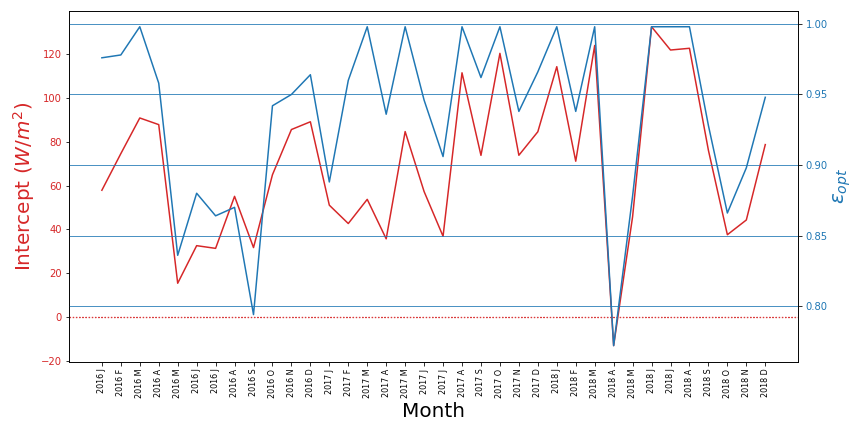
\includegraphics[scale=0.5]{slopes_AS} 
%\setlength{\belowcaptionskip}{-3ex}
%\caption{Monthly H $\Delta$T plots showing offset at $\Delta$T=0 \textbf{(a)} using simplified equation (Eq. \ref{eq_seq}). \textbf {(b)} using complete equation (Eq. \ref{eq_leq})(c). Estimated intercept (c)for each month using $H = m (T_{s} - T_{a})+ c$. Red line is intercept and blue line shows monthly $\epsilon$ obtained by minimising RMSE at Alice Springs (2016 - 2018).}
%\label{fig:mx_c1}
%\end{figure}






%conclusion future work and limitation


\section{Methods} 
\subsubsection{Research data}
\textbf{Tower data}
ECS collect micro-meteorological measurements above the surface (vegetation canopy) using towers (flux tower), following common measurement protocols \cite{baldocchi2001fluxnet}. The towers are commonly equipped with an instrument made up of pyrgeometers or radiometers to measure up-welling and down-welling shortwave and longwave radiation, which is further used to calculate net radiation (Eq. \ref{eq_Rn1}). Besides radiative fluxes, measurement at EC towers also include sensible and latent heat fluxes, net carbon dioxide exchange and a range of meteorological variables, such as air temperature, humidity and wind speed. $T_{a}$ is the air temperature measured using eddy ECS mounted above the canopy. Each flux measurement is accompanied by a flagging system and follows the agreement with second CarboEurope-IP QA/QC workshop \cite{foken2004post}. Flag 0 is designated as high data quality, and have been used in our current work. For the analysis 10 sites were selected to represent a variety of land cover types and climates (Table \ref{table:studysites}). 8 sites belong to the North Australian Tropical Transect (NATT) and 2 sites ( Yatir Forest, Brookings) are  chosen to replicate result from Holmes et.al\cite{holmes_land_2009-1}. Eddy covariance Level 3 data is obtained from http://data.ozflux.org.au/portal/pub/listPubCollections.jspx for Australian sites. The data for Brookings in obtained from ameriflux and for Yatir Forest the data was obtained using personal communication to Prof Dan Yakir's lab group as the data used in Holmes work  was from 2005 \cite{holmes_land_2009} and the current available data was an updated version of the fluxnet data.%(http://www.ntlis.nt.gov.au/metadata/export_data?metadata_id=2DBCB77120B306B6E040CD9B0F274EFE&type=html#Citation).a. %SJS: Yatir Forest is not really 

\textbf{MODIS data}
%SJS: In the methods section, you don't need to explain why you did certain things, just what and how.
%Plot scale retreived temperature is compared to MODIS daily LST data and  MODIS daily spectral emissivity are used to estimate emissivity in general approach for LST retreival. 
 Landscape- scale emissivity and LST data (MODIS product MOD11A1)  was downloaded downloaded from  NASA earth data \href{https://lpdaac.usgs.gov/}. It is a level 3 daily LST product gridded in the sinusoidal projection at a spatial resolution of 0.928 $km$ by 0.928 $km$. A tile contains 1200 x 1200 grids in 1200 rows and 1200 columns\cite{wan2007collection}. The daily LST pixel values in each granules is retrieved by the generalized split-window algorithm under clear-sky conditions and LST values are averaged by overlapping pixels in each grid with overlapping areas as weight. The downloaded data are in Hierarchical Data Format (hdf) which were converted into tagged image file format (tiff) using a python package called PyModis \cite{delucchi2014pymodis}. From tiff the files are converted into csv format. The details of data extraction and conversion can be found at $https://renkulab.io/projects/gitanjali.thakur/modis_lst_fpar/$. The dataset columns used to compare plot-scale LST and emissivity are : day time daily LST, local view time, night view time, channel 31, 32  spectral $\epsilon$ respectively. 
 %The daily LST pixel values in each granules is retrieved by the generalized split-window algorithm under clear-sky conditions through mapping all the valid clear-sky LST values onto grids in the sinusoidal projection and averaging the LST values of overlapping pixels in each grid with overlapping areas as weight..
%SJS: Remember to replace this by a zenodo link before submission.
% uncertainty estimation is defined as the  study of how uncertainty in the output of a model can be apportioned to different sources of uncertainty in input variable(e.g.,input forcing data, parameters, etc.\cite{saltelli2010variance} applied to parameter estimation.
%\subsubsection*{Study sites}
 
\begin{table}[h!]
\centering
\caption{Description of study sites}
\begin{tabular}{|p{2.5cm}|p{1.5cm}|p{2.2cm}|p{1.5cm}|p{2cm}|p{1cm}|}
 \hline
 \textbf{Study site} &\textbf{latitute, longitude} & \textbf{Landcover} & \textbf{Time-period} 
 & \textbf{longwave sensors} & \textbf{Sensor installation height (m)} \\
 \hline 
 Sturt Plains (SP) &  -17.1507, 133.3502 & Mitchell Grass & 2016-2019 & CG-2 & 4.8\\ 
 \hline
 Alice Springs (AS) &  -22.2828, 133.2493 &  Mulga woodland, hummock grassland, river red gum forest & 2016-2018 & CNR1 & 12.2\\ 
 \hline 
 Ti Tree East (TT) &  -22.2870, 133.6400 & Grassy mulga woodland, Corymbia/Triodia savanna & 2016-2018 & CNR1 & 9.9 \\
 \hline
 Howard Springs (HS) &  -12.4943, 131.1523 & Open woodland savanna & 2016-2018 & CM-7B, CG-2 & 23\\
 \hline
 Litchfield (LF) &  -13.1790, 130.7945 & Tropical savanna & 2016-2018 & CNR4 & 31 \\
 \hline
 Adelaide River (AR) & -13.0769, 131.1178 & Savanna dominated by Eucalyptus tectifica and Planchonia careya & 2006-2009 & CNR1 & 15\\
 \hline
Daly Uncleared (DU) & -14.1592, 131.3881 & Woodland savanna & 2016-2018 & NRlite & 21 \\
 \hline
 Tumbarumba (TUM) & -35.6566, 148.1517 & Wet sclerophyll & 2015-2018 &CM3 and CG3 & 70 \\
 \hline
Brookings (BR) & 44.352, 96.840 & Cropland & 2005 & pyrgeometers\cite{guillevic2017land}& NA
 \\
 \hline 
 Yatir Forest (YF) & 35.052, 31.345 & Evergreen needleleaf forest & 2005 & pyrgeometers\cite{guillevic2017land}
 & NA\\
 \hline 
\end{tabular}
\label{table:studysites}
\end{table}


\textbf{Site-specific approach}
%The above expression for sensible heat (Eq. \ref{eq_H}) is based on two assumptions: (1) $H$ is directly proportional to the near-surface temperature gradient; and (2) the temperature gradient is represented by a difference in radiometric surface temperature and air temperature ($T_{s} - T_{a}$).
%Range of emissivity is selected starting from the maximum possible emissivity of grey body (0.998) and with each iteration and emissivity is reduced in a step size of 0.002 untill $T_{s} - T_{a}$ is 0 at $H = 0$. The emissivity at which the regression between $H(\Delta$ T) passed through zero and the root mean square error is minimum ( see methods for detail) is called as optimum emissivity. 
This approach was initially proposed by Holmes\cite{holmes_land_2009-1} to estimate plot-scale $\epsilon$ using short equation with $H, R_{lup},T_{a}$. In  present work we have used both long equation (Eq. \ref{eq_Tleq}) and short equation (Eq. \ref{eq_Tleq}) to estimate $\epsilon$
The prime variable used in the study are $H, R_{lup}, R_{ldwn},T_{a}$ and the ancillary variable are $R_{n}$ and wind speed (Ws) are used to filter the data for analysis. The filtering condition were $R_{n} > 25 Wm^-2$) and wind speed ($Ws > 2ms^-1$)\cite{holmes_land_2009}. Plot scale emissivity is derived by segregating each month data satisfying the filtering criteria. For estimating $T_{s}$ from longwave measurement($R_{lup},R_{ldwn}$) a predefined range of $\epsilon$ is chosen starting from 0.998 and is reduced at a step size of 0.002. For each month data $H (T_{s} - T_{a})$ linear regression is performed using scipy $https://docs.scipy.org/doc/scipy-0.14.0/reference/generated/scipy.stats.linregress.html$. The
$R^2$ is checked and months where $R^{2} > 0.5$ (i.e substantial part of variance in H is explained by $T_{s} -T_{a}$) is chosen for $\epsilon$ estimation. To obtain $epsilon$ regression line of $H, \Delta T$ is forced through origin ( at $T_{s} - T_{a} = 0 $  $H=0$) by minimising  the RMSE. An illustration plot for RMSE and $\epsilon$ is shown in \textbf{SI5}. The  $\epsilon_{plot}$ is obtained for each month using both long Eq.(\ref{eq_Tleq}) and short equation Eq.(\ref{eq_Tseq}) and  termed as $\epsilon_{seq}$ and $\epsilon_{leq}$ as shown in Fig. \ref{fig:flow_chart}b. In the next step instead of forcing the $ H vs \Delta T$ plot through origin robust linear regression is used, which allowed an offset in monthly $H (\Delta T)$ plots. The plot-scale $\epsilon$ was obtained by minimising RMSE as explained before. Plot-scale LST estimated using plot-scale $\epsilon$ was compared to landscape-scale MODIS LST. Monthly tower based longwave measurement at study sites corresponding to TERRA daily time of pass was obtained using linear interpolation. TERRA (satellite) overpasses at local solar time between 10:30 am to 12 pm in ascending mode \cite{guillevic2017land}. Plot-scale LST (( $T_{leq}$ and $T_{seq}$) was obtained using interpolated day time longwave measurement and crossponding month plot-scale $\epsilon$ using Eq. (\ref{eq_Tleq}), Eq. (\ref{eq_Tseq}) . Plot-scale daily LST is compared to MODIS LST in terms of mean, bias, RMSE and $R^2$ using a robust linear regression model(scipy stat model) as shown in Fig. \ref{fig:flow_chart}a. The goodness of fit between plot-scale and landscape-scale LST was determined by looking at ($R^2$) as shown in Fig. \ref{fig:flow_chart}b. The bias is estimated as mean of deviation between daily MODIS LST and ground based $T_{s}$ ($T_{leq,seq} - T_{MODIS}$). See SI table for data sources and acronyms in \textbf{SI1}

\textbf{General Approach}
In this approach we estimate Landscape-scale $\epsilon$ (Broadband) is  estimated using MODIS spectral $\epsilon$ as shown\cite{bahir_evaluation_2017}
\begin{equation}\label{eq_emodis}
\epsilon_{MODIS}= 0.4587 \epsilon_{31} + 0.5414 \epsilon_{32}
\end{equation}
Tower based longwave measurement ($R_{lup}, R_{ldwn}$) passing the filtering criteria (as mentioned in site- specific approach) along with MODIS based $\epsilon$ was used  to invert LST using Eq. (\ref{eq_Tleq}) and  Eq. (\ref{eq_Tseq}). Plot-scale LST estimated using MODIS based $\epsilon$ was compared to landscape-scale MODIS LST using a robust linear regression as done in site specific approach as shown in Fig. (\ref{fig:flow_chart}a).

%In order to avoid the  error in  measured longwave fluxes, quality flag filter has been applied to the datasets used for LST retreivals. The remaining speculated source of error can be MODIS based surface emissivity, therefore another method of broadband emissivity estimation is used

 %SJS: Could you re-formulate to focus on what you did and how?
  
%\hyperlink{https://earthdata.nasa.gov/earth-observation-data/near-real-time/download-nrt-data/modis-nrt#ed-modis-terra-aqua-c6}.
%SJS: downloaded from where? 
%I would just use acronyms here and then provide a table with the data sources related to the acronyms.

\textbf{Uncertainty estimation}
The uncertainty in plot-scale $\epsilon$ due to error is observed fluxes is estimated. In first step, the error bounds of each input variables ($ H, R_{lup}, R_{ldw}, T_{a}$) is assumed. The error bounds for $R_{lup}  R_{ldwn}$ are -5 to 5 W m$^{-2}$ \cite{trenberth2012tracking}, for $H$ is -20 to 20 W m$^{-2}$ and for $T_{a}$ it is -1 to 1 K \cite{foken2008energy}. Uniformly distributed samples within error bounds are generated using saltelli sampling scheme\cite{saltelli2017new} using python based package name SALIB. Each error samples are added to the  monthly segregated measured fluxes. The plot-scale $\epsilon$ is estimated for the fluxes with added uncertainty (error sample) as explained in site specific approach. The obtained range of plot-scale $\epsilon$ is reported as uncertainity in emissivity . The plot-scale $\epsilon$ uncertainty  with uncertainty in $R_{lup}, R_{ldw}$ is used to calculate the uncertainty in hourly LST using short equation Eq. \ref{eq_Tseq} and long equation Eq.\ref{eq_Tleq} as shown in Fig. \ref{fig:eps_unc1}b,c. 
. 
 
\begin{figure}[h!]
\begin{subfigure}{.5\textwidth}
\centering
\scalebox{1}{
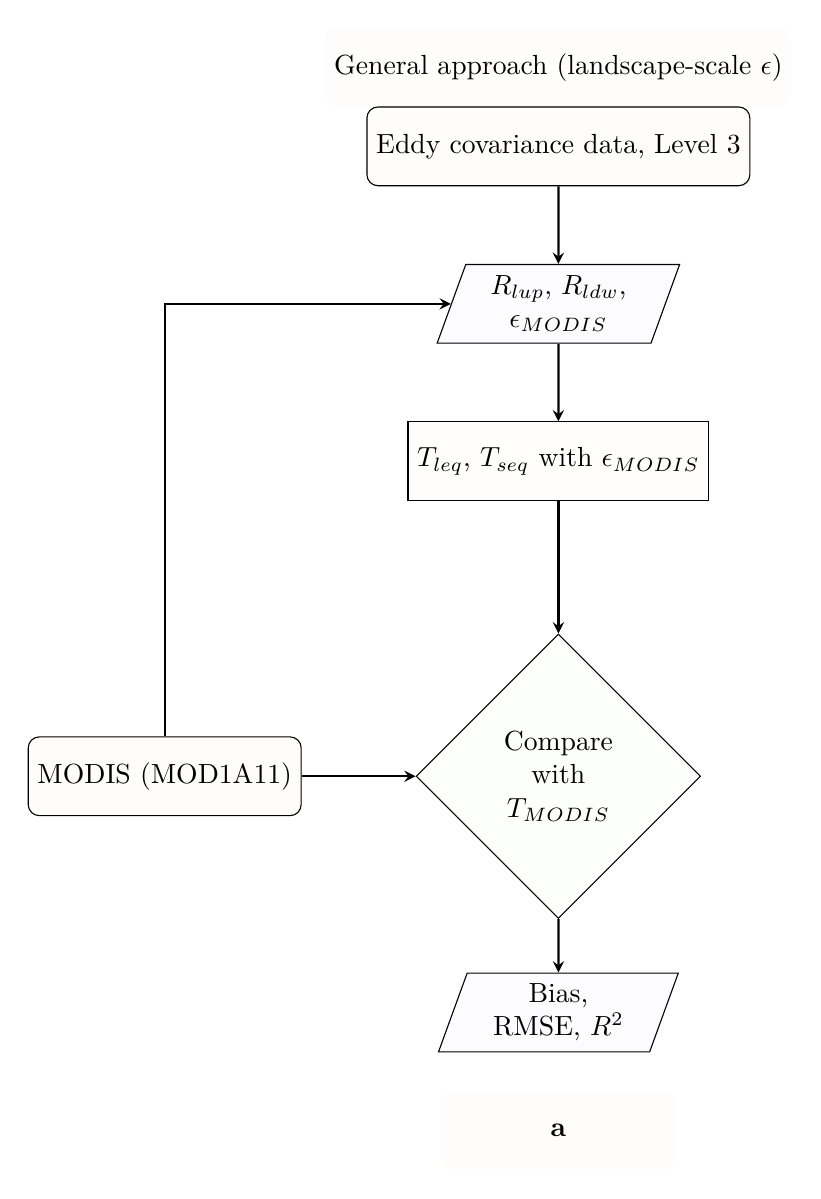
\begin{tikzpicture}[node distance=2cm]
\node (txt) [textbox] {General approach (landscape-scale $\epsilon$)};
\node (start) [startstop,yshift=-1cm] {Eddy covariance data, Level 3};
\node (in1) [io, below of=start] {$R_{lup}$, $R_{ldw}$, $\epsilon_{MODIS}$};
\node (pro1) [process, below of=in1] {$T_{leq}$, $T_{seq}$ with $\epsilon_{MODIS}$};
\node (dec1) [decision, below of=pro1, yshift=-2cm] {Compare with $T_{MODIS}$};
\node (start1) [startstop, left of=dec1, xshift=-3cm] {MODIS (MOD1A11)};
\node (out1) [io, below of=dec1,yshift=-1cm] {Bias, RMSE, $R^{2}$};
%\node (stop) [startstop, below of=out1] {Stop};
\draw [arrow] (start) -- (in1);
\draw [arrow] (in1) -- (pro1);
\draw [arrow] (pro1) -- (dec1);
\draw [arrow] (start1) -- node[anchor=east] {} (dec1);
\draw [arrow] (start1) |- (in1);
\draw [arrow] (dec1) -- (out1);
\node (txt1) [textbox, below of=out1,yshift= 0.5cm] {\textbf{a}};
\end{tikzpicture}}
\end{subfigure}
\begin{subfigure}{.5\textwidth}
\centering
\scalebox{0.75}{
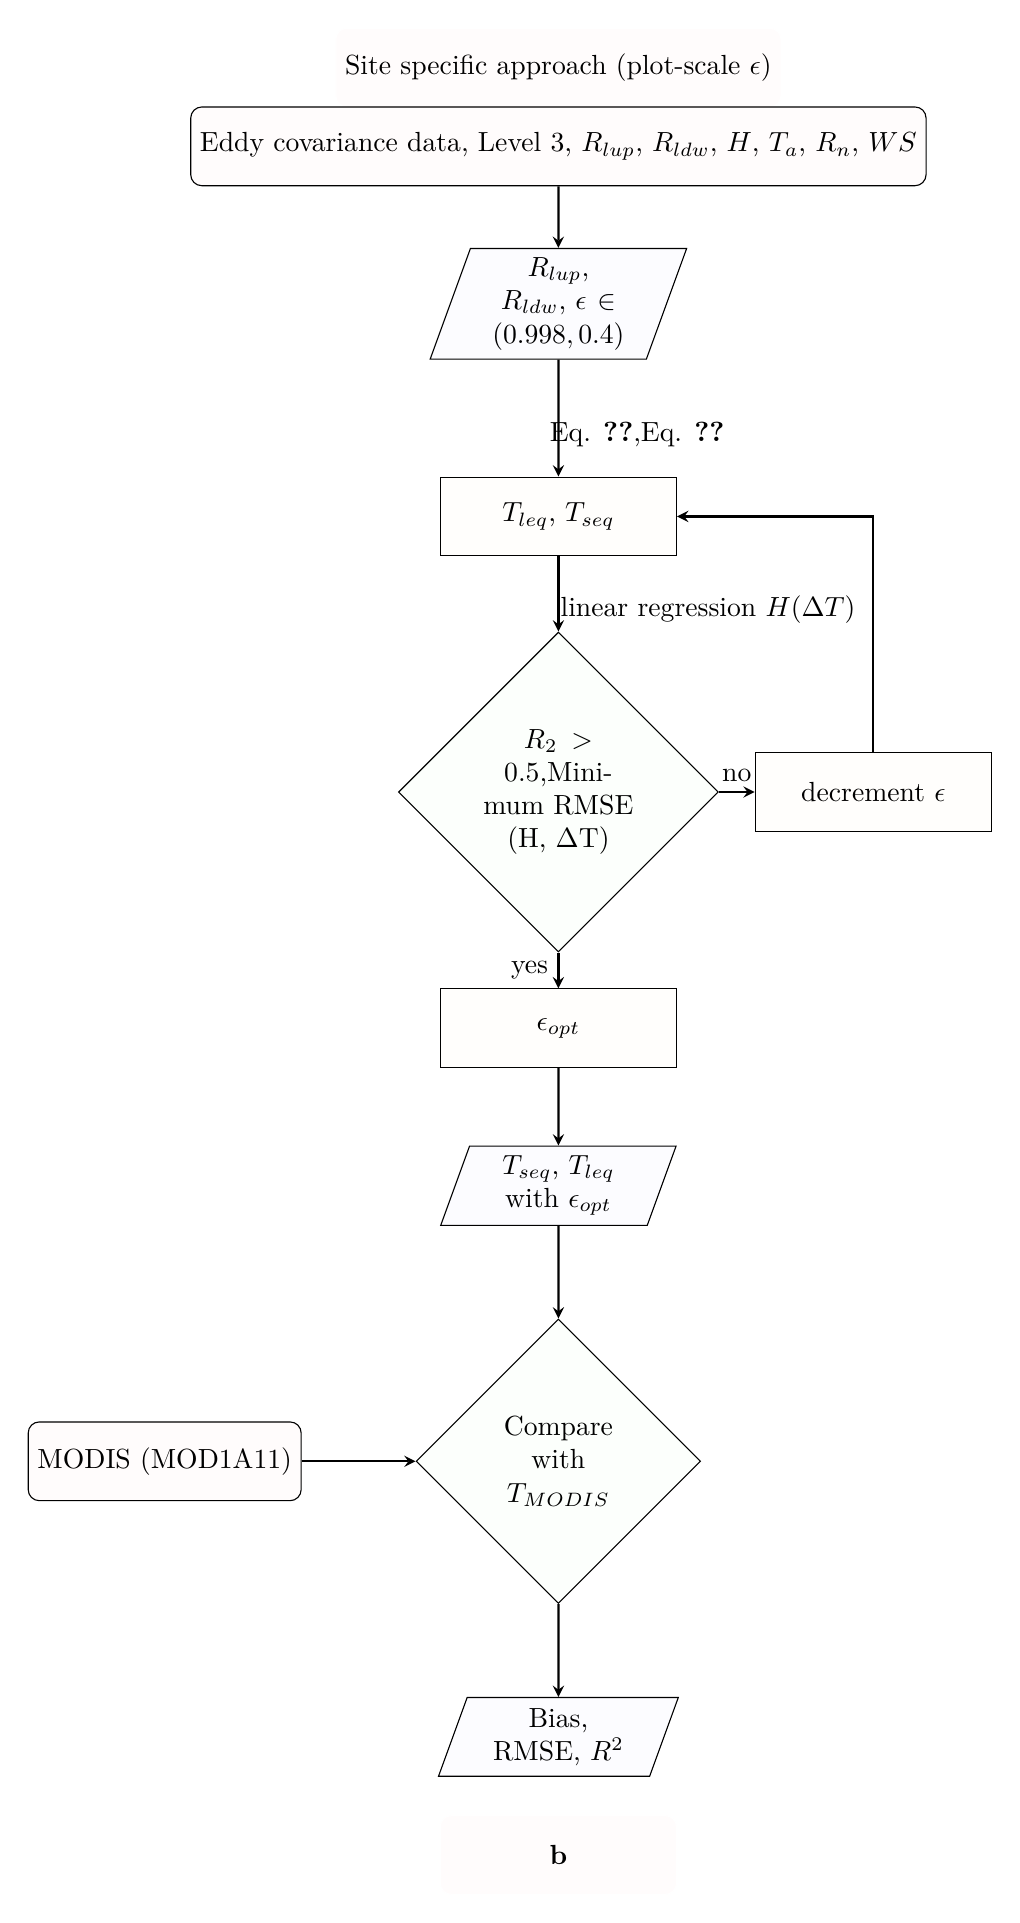
\begin{tikzpicture}[node distance=2cm]
\node (txt) [textbox] {Site specific approach (plot-scale $\epsilon$)};
\node (start) [startstop, yshift= -1 cm] {Eddy covariance data,  Level 3, $R_{lup}$, $R_{ldw}$, $H$, $T_a$, $R_n$, $WS$};
node[anchor=north] {yes} (start);
\node (in1) [io, below of=start] {$R_{lup}$, $R_{ldw}$, $\epsilon \in ({0.998, 0.4})$};
\node (pro1) [process, below of=in1, yshift=-0.7cm] {$T_{leq}$, $T_{seq}$};
\node (dec1) [decision, below of=pro1, yshift=-1.5cm] {$R_{2} > 0.5$,Minimum RMSE (H, $\Delta$T)} ;
\node (pro2a) [process, below of=dec1, yshift=-1cm] {$\epsilon_{opt}$};
\node (pro2b) [process, right of=dec1, xshift=2cm] {decrement $\epsilon$};
\node (out1) [io, below of=pro2a] {$T_{seq}$, $T_{leq}$ with $\epsilon_{opt}$};
\node (dec2) [decision, below of=out1, yshift=-1.5cm] {Compare with $T_{MODIS}$};
\node (start1) [startstop, left of=dec2, xshift=-3cm] {MODIS (MOD1A11)};
\node (out2) [io, below of=dec2,yshift=-1.5cm] {Bias, RMSE, $R^{2}$};
%\node (stop) [startstop, below of=out1] {Stop};
\draw [arrow] (start) -- (in1);
\draw [arrow] (in1) --  node[anchor=south,xshift=1cm, yshift=-0.5cm] {Eq. \ref{eq_Tleq},Eq. \ref{eq_Tseq}} (pro1);
\draw [arrow] (pro1) -- node[anchor=south,xshift=1.9cm, yshift=-0.5cm] {linear regression $H(\Delta T)$} (dec1);
\draw [arrow] (dec1) -- node[anchor=east] {yes} (pro2a);
\draw [arrow] (dec1) -- node[anchor=south] {no} (pro2b);
\draw [arrow] (pro2b) |- (pro1);
\draw [arrow] (pro2a) -- (out1);
\draw [arrow] (out1) -- (dec2);
\draw [arrow] (dec2) -- (out2);
\draw [arrow] (start1) -- node[anchor=east]{} (dec2);
\node (txt2) [textbox,below of=out2,yshift= 0.5cm] {\textbf{b}};
\end{tikzpicture}}
\end{subfigure}
\caption{Schematic representation of  steps followed for plot scale LST retreival using eddy covariance measurement(a) Landscape emissivity and longwave measurement and compared to Landscape-scale LST($T_{MODIS}$).(b) Plot-scale emissivity estimation using observed $H, R_{ldwn},R_{lup}$ and plot-scale LST is estimated using plot-scale $\epsilon$ is compared to landscape-scale emissivity. The $R^{2}$, RMSE, Bias are mentioned in Fig. (\ref{fig:LST local and MODIS})}
\label{fig:flow_chart}
\end{figure}





\section{Acknowledgements}
We would like to thank Dr. Maik Renner for pointing us to the work by Holmes et al. and Dan Yakir's lab for providing Yatir Forest data and helpful discussions. We are also grateful to Thomas Foken, Jason Beringer, Lindsay Hutley, Mauro Sulis for insightful discussions and Remko Nijzink for his help in programming and RENKU. This work is supported by the Luxembourg National Research Fund (FNR) ATTRACT programme (WAVE, A16/SR/11254288).

%Acknowledgements should be brief, and should not include thanks to anonymous referees and editors, or effusive comments. Grant or contribution numbers may be acknowledged.

%\bibliographystyle{abbrvnat}


\bibliography{lstpaper,not_indexed_ref}
%\bibliography{not_indexed_ref}

\section{Supplementary Information}
%SJS: Should the below figures be part of the pdf, or separate?
%GT: it should be separate
\subsection*{SI1. Abbreviation list}
\begin{table}[h!]

\centering
\caption{Abbreviation list}
\begin{tabular}{p{2.5cm} p{3.0cm} p{3.0cm}}

%\begin{tabular}{|c|c|} 
\hline

Symbol & Description & Unit\\

\hline
$R_{net}$ & Net radiation & W m$^{-2}$ m \\
$H$ & Sensible heat flux & W m$^{-2}$ \\
$LE$ & Latent heat flux & W m$^{-2}$ \\
$G$ & Ground heat flux & W m$^{-2}$ \\
$R_{lem}$ & Emittied longwave radiation & W m$^{-2}$ \\
$\epsilon$ & Surface emissivity & (-)\\
$\sigma$ & Stefan-Boltzmann constant & W m$^{-2}$K$^{-4}$\\
$T_{s}$ & Surface temerature & K\\
$R_{sdwn}$ & Down-welling shortwave & W m$^{-2}$\\
$R_{ldwn}$ & Down-welling longwave & W m$^{-2}$\\
$R_{sref}$ & Reflected shortwave & W m$^{-2}$\\
$\alpha$ & Surface albedo & (-)\\
$m$ & Aerodynamic conductance to heat transport & $(m/s)$\\
$\epsilon$ 31 & Spectral emissivity for wavelength of 11 $\mu$m & (-) \\
$\epsilon$ 32 & Spectral emissivity for wavelength of 12 $\mu$m & (-)  \\
BADAM & Ameriflux dataset & (-) \\
TERRA & NASA scientific research satellite & (-)  \\
NATT & North Australian Tropical Transect & (-) \\

\hline
\end{tabular}
\label{table:SI2}
\end{table}

\subsection*{SI2. Comparison table of plot-scale LST with landscape LST using landscape and plot-scale $\epsilon$}

\begin{table}[h!]
\centering
\begin{tabular}{|c|c|c|c|c|c|c|c|c|c|c|c|}
 \hline
 \multirow{3}{*}{\textbf{Sites}} & \multicolumn{5}{c}{Landscape-scale $\epsilon$} \vline & \multicolumn{6}{c}{Plot-scale $\epsilon$} \vline \\\cline{2-12}
&  \multirow{2}{*} {$\epsilon$} &  \multicolumn{2}{c}{seq} \vline &  \multicolumn{2}{c}{leq} \vline 
&  \multicolumn{3}{c}{seq} \vline &  \multicolumn{3}{c}{leq}\vline\\ \cline{3-12}
& & $R^2$ & bias & $R^2$ & bias & opt $\epsilon$ & $R^2$ & bias & opt $\epsilon$ & $R^2$ & bias  \\
\hline
SP & 0.974 & 0.80 & -3.67 & 0.81 & -4.61 & 0.96 & 0.81 & -3.0 & 0.85 & 0.82 & -1.91\\
\hline 
AS & 0.974 & 0.93 & -4.78  &0.93  & -6.31 & 0.96 & 0.93  & -3.4 & 0.82 & 0.93 & -1.92  \\ 
 \hline 
TT & 0.974 & 0.55 & -6.76 & 0.57 & -8.30 & 0.95 & 0.58  & -5.06 & 0.80 & 0.52 & -4.02 \\
 \hline
HS & 0.985 & 0.16 & -8.89 & 0.16 & -9.90 & 0.92 & 0.21  & -4.78 & 0.6 & 0.22 & -2.47\\
 \hline
LF & 0.985 & 0.40 & -10.0 & 0.41 & -11.0 & 0.92 & 0.40  & -4.41 & 0.6 & 0.41 & -2.57 \\
 \hline
AR & 0.985 & 0.18 & -2.61 & 0.27 & -3.51 & 0.997 & 0.23  & -2.93 & 0.96 & 0.252 & -2.98\\
 \hline
 DU & 0.985 & 0.80 & -3.67 & 0.81 & -4.61 & 0.99 & 0.428  & -3.682 & 0.985 & 0.425 & -3.926\\
 \hline
TUM & 0.983 & 0.82 &-2.27& 0.84 & -2.10 & 0.99 & 0.89  & 0.99 & 0.97 & 0.89 & 1.93\\
 \hline
BR &0.983 &0.937  &0.525 & 0.937 &-0.195  & 0.98 & 0.917 & 1.87 & 0.82 & 0.895 & 2.72\\
 \hline
YA & 0.974 & 0.855 &-2.081 & 0.855 & -3.45 & 0.97& 0.522 &-4.517 & 0.93 & 0.793 & -0.582\\
 \hline
\end{tabular}
 \caption{ Comparison of plot-scale LST with landscape-scale daytime LST (MODIS, MODA001) at TERRA daily time of pass. Plot scale LST is obtained using landscape-scale emissivity (MODIS $\epsilon$) and plot-scale emissivity (Optimum $\epsilon$) at study sites. The reported plot-scale emissivity are median values and landscape emissivity are MODIS based. Bias is defined as mean of $T_{s} - T_{MODIS}$, $R^{2}$ is coefficient of determination between plot-scale LST in comparison to landscape-scale LST. The site acronyms can be found in Table {\ref{table:studysites}}
 %SJS: What do you mean by bias, $R^{2}$ and median of monthly emissivity? Bias and $R^{2}$ refer to plot-scale LST in comparison to MODIS LST, right? Please clarify. Also need to explain where to find site acronyms explained, what seq and leq means. Maybe instead of MODIS epsilon and Optimum epsilon, we could call it landscape-scale and plot-scale or satellite-based vs. locally estimated? Can you clarify in the caption that only LST estimates for the times of satellite overpasses were used?
 } 
\label{table:SI2_optlstandmod}  
\end{table}




\subsection*{SI3. Emissivity estimation at Howards spring and positive $T_{s}-T_{a}$ }
\begin{figure}[h!]
	\begin{subfigure}{\textwidth}
		\begin{overpic}[width=0.45\textwidth]{hS_seq_2018-05} % ,grid,tics=10
			\put (18,61){\textbf{a}}
		\end{overpic}
		\begin{overpic}[width=0.45\textwidth]{hS_le_2018-05} % ,grid,tics=10
			\put (18,61){\textbf{b}}
		\end{overpic}
	\end{subfigure}
	\setlength{\belowcaptionskip}{-3ex}
	\caption{$ H and \Delta T$ plots at Howards Spring with optimised emissivity}
	\label{fig:hs_hdt}
\end{figure}
 
\subsection*{SI4.$T_{s}$ sensitivity to $\epsilon$ at Alice spring and Tumbarumba}
 \begin{figure}[h!]
\centering
\begin{subfigure}{.5\textwidth}
  \centering
  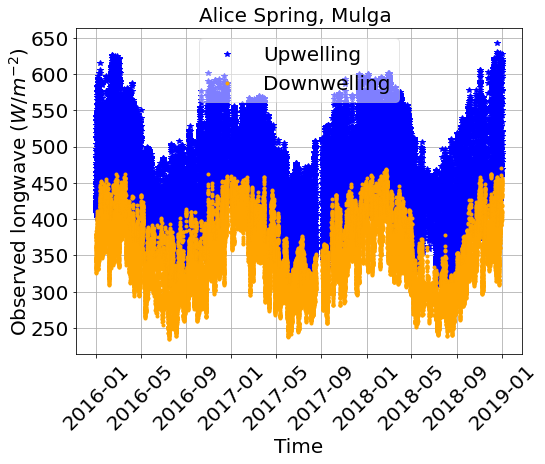
\includegraphics[width=.95\linewidth]{Alice_spring_longw.png}
  \caption{Alice Springs}
  
\end{subfigure}%
\begin{subfigure}{.5\textwidth}
  \centering
  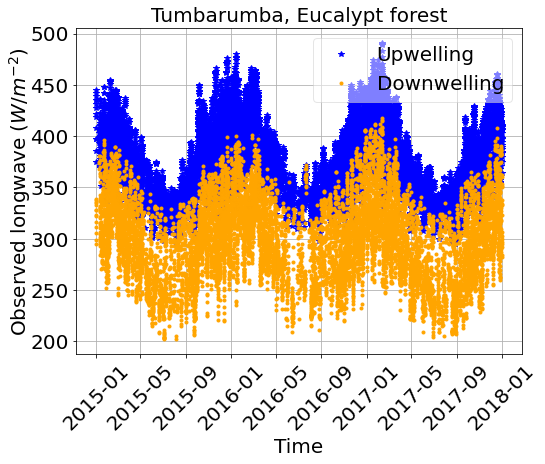
\includegraphics[width=.95\linewidth]{TUM_longw}
  \caption{Tumbarumba}
\end{subfigure}
\setlength{\belowcaptionskip}{-3ex}
\caption{Measured up-welling and down-welling longwave timeseries}
\label{fig:longwave}
\end{figure}
In general the broadband emissivity range for a land cover can vary between 0.87 to 0.98\cite{jin_improved_2006}. The noontime measured longwave for two contrasting landcover types (semi-arid mulga, tropical savanna woodland) are used to quantify the sensitivity of LST to emissivity as shown in Fig. (\ref{fig:LST sensitivity to emissivity}).
\begin{figure}[h!]
\centering
\begin{subfigure}{.5\textwidth}
  \centering
  \includegraphics[width=.95\linewidth]{{Alice_spring_Ts_sensitivity_2005}}
  \caption{}
  \label{fig:sub1}
\end{subfigure}%
\begin{subfigure}{.5\textwidth}
  \centering
  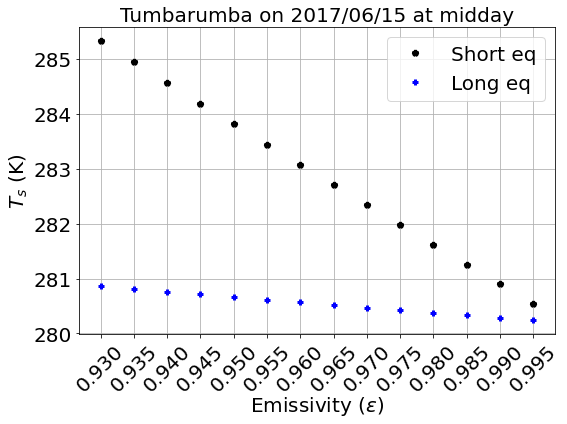
\includegraphics[width=.95\linewidth]{Tum_Ts_sensitivity_2016}
  \caption{}
  \label{fig:sub2}
\end{subfigure}
\setlength{\belowcaptionskip}{-3ex}
\caption{Sensitivity of LST estimated using two equations to the range of Broadband emissivity The black dots and blue Stars depicts LST using simplified (Eq. \ref{eq_seq}) and complete (Eq. (\ref{eq_leq}). Midday longwave measurement for 15June, 2016 at Alice Springs and Tumbarumba is used}
\label{fig:LST sensitivity to emissivity}
\end{figure}







\subsection*{SI5.RMSE and Epsilon}
\label{Subsection:RMSE}
\begin{figure}[h!]
\centering
\begin{subfigure}{.5\textwidth}
  \centering
  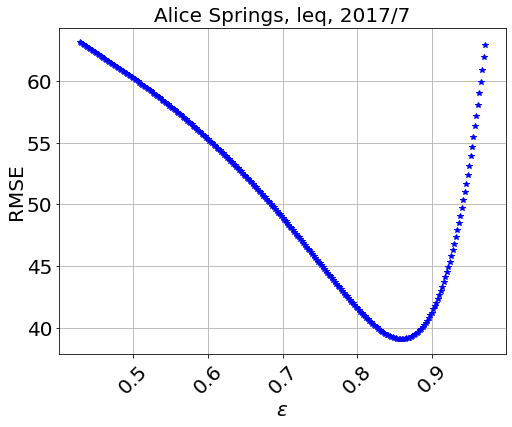
\includegraphics[width=.95\linewidth]{AS_RMSE_2018}
  \caption{Alice Springs}
  
\end{subfigure}%
\begin{subfigure}{.5\textwidth}
  \centering
  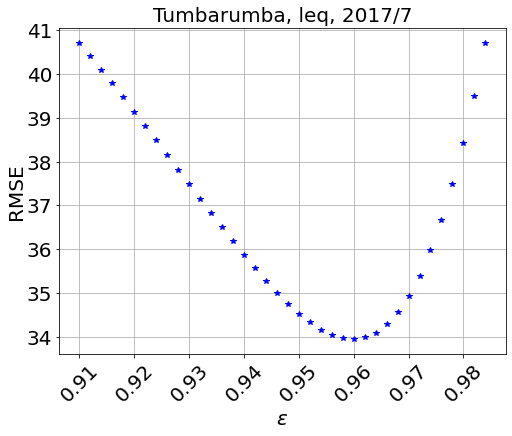
\includegraphics[width=.95\linewidth]{tum_RMSE_2017}
  \caption{Tumbarumba}
\end{subfigure}
\setlength{\belowcaptionskip}{-3ex}
\caption{RMSE and emissivity curve}
\label{fig:rmse_eps}
\end{figure}

\subsection*{SI6.Energy imbalance and observed fluxes}
\label{Subsection:wnimb}
\begin{figure}[h!]
  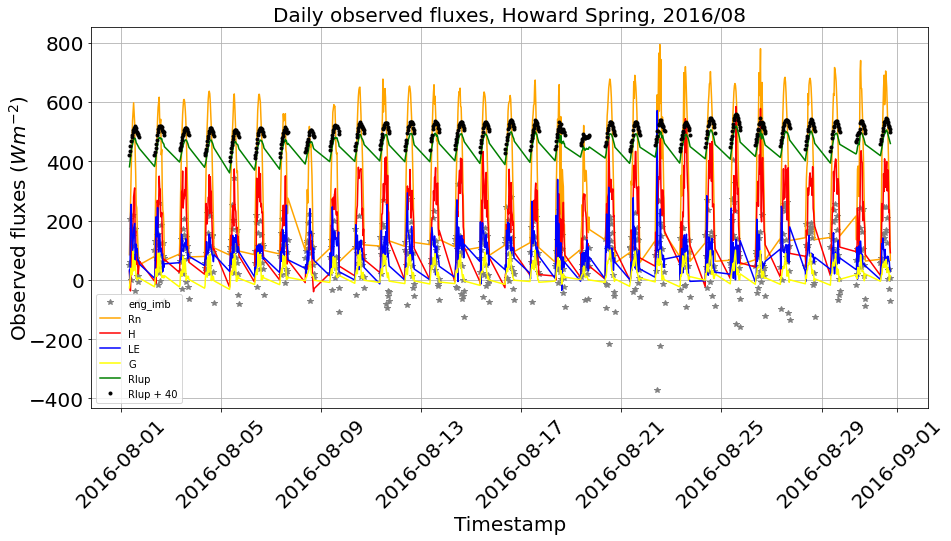
\includegraphics[scale=0.5]{hs_enb.png}
  \caption{Measured fluxes and estimated energy imbalance at Howard springs for 2016/08}
  \label{fig:wninb}
  \end{figure}

\subsection*{SI7.H and intercept}
\label{Subsection:intercept}
\begin{figure}[h!]
  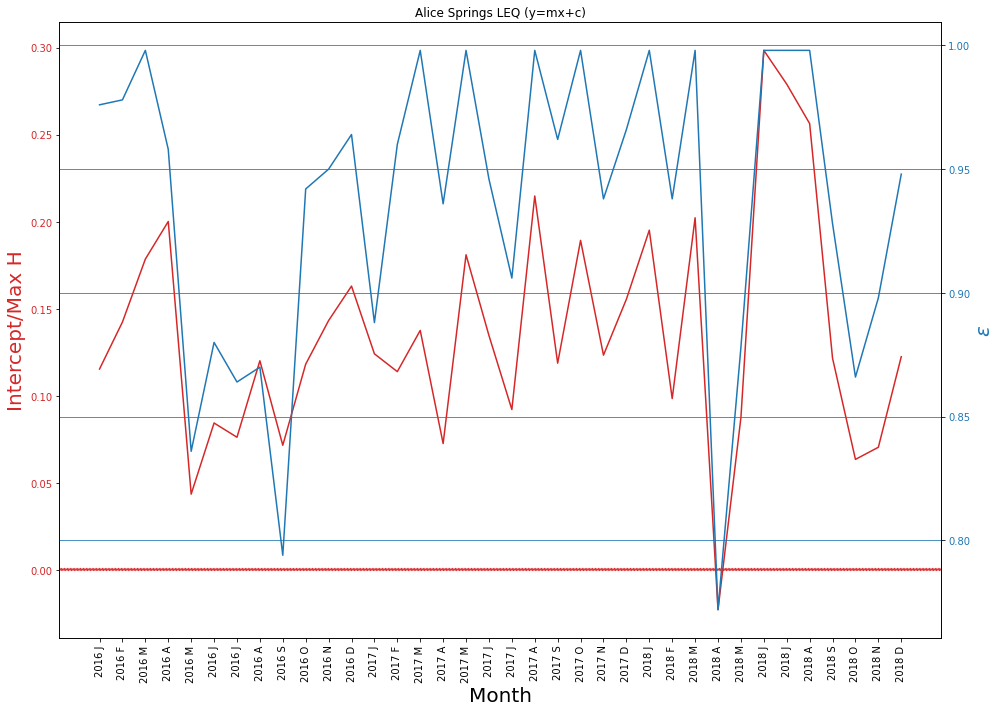
\includegraphics[scale=0.5]{Plots/as_mx+c.png}
  \caption{Monthly H $\Delta$T plots showing offset at $\Delta$T=0 \textbf{(a)} using simplified equation (Eq. \ref{eq_seq}). \textbf {(b)} using complete equation (Eq. \ref{eq_leq})(c). Estimated intercept (c)for each month using $H = m (T_{s} - T_{a})+ c$. Red line is intercept and blue line shows monthly $\epsilon$ obtained by minimising RMSE at Alice Springs (2016 - 2018).}
  \label{fig:yr_intrc}
  \end{figure}
%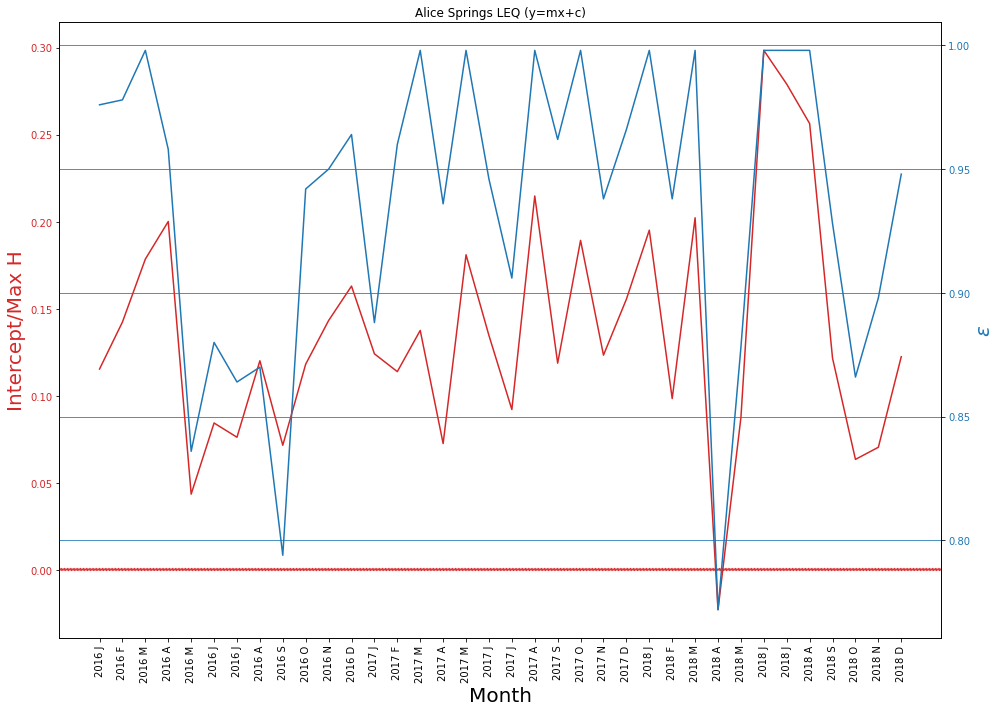
\includegraphics[scale=0.5]{Plots/as_mx+c.png} 

%\caption{








\end{document}

\section*{Results}

Up to three levels of \textbf{subheading} are permitted. Subheadings should not be numbered.

\subsection*{Subsection}

Example text under a subsection. Bulleted lists may be used where appropriate, e.g.

\begin{itemize}
\item First item
\item Second item
\end{itemize}

\subsubsection*{Third-level section}
 
Topical subheadings are allowed.

\section*{Discussion}

The Discussion should be succinct and must not contain subheadings.

\section*{Methods}

Topical subheadings are allowed. Authors must ensure that their Methods section includes adequate experimental and characterization data necessary for others in the field to reproduce their work.

\bibliography{sample}

\noindent LaTeX formats citations and references automatically using the bibliography records in your .bib file, which you can edit via the project menu. Use the cite command for an inline citation, e.g.  \cite{Hao:gidmaps:2014}.

For data citations of datasets uploaded to e.g. \emph{figshare}, please use the \verb|howpublished| option in the bib entry to specify the platform and the link, as in the \verb|Hao:gidmaps:2014| example in the sample bibliography file.

\section*{Acknowledgements (not compulsory)}

Acknowledgements should be brief, and should not include thanks to anonymous referees and editors, or effusive comments. Grant or contribution numbers may be acknowledged.

\section*{Author contributions statement}

Must include all authors, identified by initials, for example:
A.A. conceived the experiment(s),  A.A. and B.A. conducted the experiment(s), C.A. and D.A. analysed the results.  All authors reviewed the manuscript. 

\section*{Additional information}

To include, in this order: \textbf{Accession codes} (where applicable); \textbf{Competing interests} (mandatory statement). 

The corresponding author is responsible for submitting a \href{http://www.nature.com/srep/policies/index.html#competing}{competing interests statement} on behalf of all authors of the paper. This statement must be included in the submitted article file.

\begin{figure}[h!]
\centering
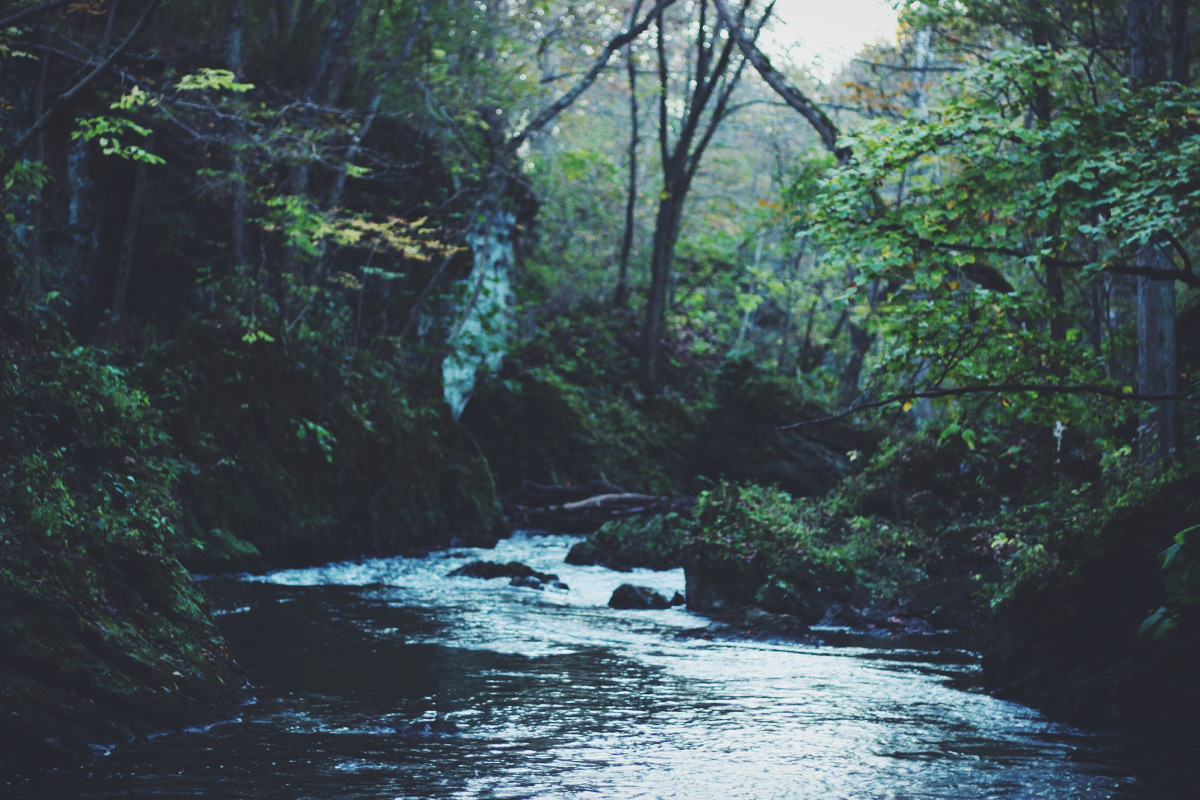
\includegraphics[width=\linewidth]{stream}
\caption{Legend (350 words max). Example legend text.}
\label{fig:stream}
\end{figure}

\begin{table}[ht]
\centering
\begin{tabular}{|l|l|l|}
\hline
Condition & n & p \\
\hline
A & 5 & 0.1 \\
\hline
B & 10 & 0.01 \\
\hline
\end{tabular}
\caption{\label{tab:example}Legend (350 words max). Example legend text.}
\end{table}

Figures and tables can be referenced in LaTeX using the ref command, e.g. Figure \ref{fig:stream} and Table \ref{tab:example}.
\begin{figure}[h!]
\centering
\begin{subfigure}{.5\textwidth}
  \centering
  \includegraphics[width=.95\linewidth]{AS_le_2017-06}
  \caption{H vs Ts -Ta using complete equation for june 2017}
  \label{fig:HDTAsleq}
\end{subfigure}%
\begin{subfigure}{.5\textwidth}
  \centering
  \includegraphics[width=.95\linewidth]{AS_se_2017-06}
  \caption{H vs Ts -Ta using simplified  equation }
  \label{fig:sub2}
\end{subfigure}
\setlength{\belowcaptionskip}{-3ex}
\caption{H vs DT plots using MODIS emissivity}
\label{fig:HDTasseq}
\end{figure}

\end{document}




\end{document}

\section*{Results}

Up to three levels of \textbf{subheading} are permitted. Subheadings should not be numbered.

\subsection*{Subsection}

Example text under a subsection. Bulleted lists may be used where appropriate, e.g.

\begin{itemize}
\item First item
\item Second item
\end{itemize}

\subsubsection*{Third-level section}
 
Topical subheadings are allowed.

\section*{Discussion}

The Discussion should be succinct and must not contain subheadings.

\section*{Methods}

Topical subheadings are allowed. Authors must ensure that their Methods section includes adequate experimental and characterization data necessary for others in the field to reproduce their work.

\bibliography{sample}

\noindent LaTeX formats citations and references automatically using the bibliography records in your .bib file, which you can edit via the project menu. Use the cite command for an inline citation, e.g.  \cite{Hao:gidmaps:2014}.

For data citations of datasets uploaded to e.g. \emph{figshare}, please use the \verb|howpublished| option in the bib entry to specify the platform and the link, as in the \verb|Hao:gidmaps:2014| example in the sample bibliography file.

\section*{Acknowledgements (not compulsory)}

Acknowledgements should be brief, and should not include thanks to anonymous referees and editors, or effusive comments. Grant or contribution numbers may be acknowledged.

\section*{Author contributions statement}

Must include all authors, identified by initials, for example:
A.A. conceived the experiment(s),  A.A. and B.A. conducted the experiment(s), C.A. and D.A. analysed the results.  All authors reviewed the manuscript. 

\section*{Additional information}

To include, in this order: \textbf{Accession codes} (where applicable); \textbf{Competing interests} (mandatory statement). 

The corresponding author is responsible for submitting a \href{http://www.nature.com/srep/policies/index.html#competing}{competing interests statement} on behalf of all authors of the paper. This statement must be included in the submitted article file.

\begin{figure}[h!]
\centering
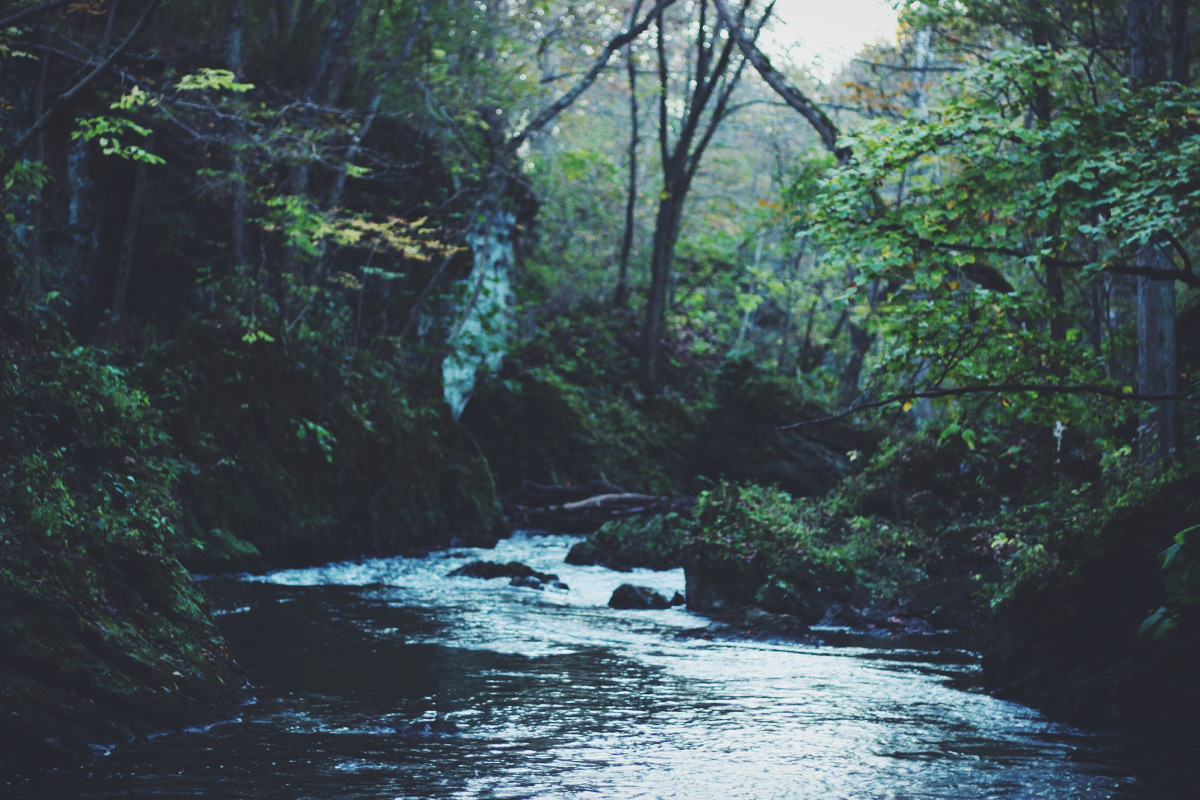
\includegraphics[width=\linewidth]{stream}
\caption{Legend (350 words max). Example legend text.}
\label{fig:stream}
\end{figure}

\begin{table}[ht]
\centering
\begin{tabular}{|l|l|l|}
\hline
Condition & n & p \\
\hline
A & 5 & 0.1 \\
\hline
B & 10 & 0.01 \\
\hline
\end{tabular}
\caption{\label{tab:example}Legend (350 words max). Example legend text.}
\end{table}

Figures and tables can be referenced in LaTeX using the ref command, e.g. Figure \ref{fig:stream} and Table \ref{tab:example}.
\begin{figure}[h!]
\centering
\begin{subfigure}{.5\textwidth}
  \centering
  \includegraphics[width=.95\linewidth]{AS_le_2017-06}
  \caption{H vs Ts -Ta using complete equation for june 2017}
  \label{fig:HDTAsleq}
\end{subfigure}%
\begin{subfigure}{.5\textwidth}
  \centering
  \includegraphics[width=.95\linewidth]{AS_se_2017-06}
  \caption{H vs Ts -Ta using simplified  equation }
  \label{fig:sub2}
\end{subfigure}
\setlength{\belowcaptionskip}{-3ex}
\caption{H vs DT plots using MODIS emissivity}
\label{fig:HDTasseq}
\end{figure}

\end{document}
